\documentclass[14pt, a4paper]{bsu}

\usepackage{titlesec}
\usepackage{titling}
\usepackage{verbatim}
\usepackage{csquotes}
\usepackage{longtable}
\usepackage{subcaption}
\usepackage[backend=biber, style=numeric, sorting=title]{biblatex}

\DeclareSortingTemplate{title}{
  \sort{
    \field{title}
  }
}

\addbibresource{references.bib}
\DeclareNameAlias{sortname}{family-given}

\title{Оценка влияния солнечной активности на работу бортовых систем
  низкоорбитальных спутников с использованием алгоритма машинного обучения
XGBoost и построения графа связности}
\author{Глеба Е. М., Баранова В. С.}
\date{\today}

\graphicspath{{../img}{../mermaid}}

\begin{document}

\hyphenation{Sat-NOGS}
\hyphenation{Xg-Boost}
\hyphenation{xg-boost}
\hyphenation{Po-la-ris}
\hyphenation{multi-purpose}
\hyphenation{Con-fe-re-nce}
\hyphenation{Hu-man-kind}
\hyphenation{Ja-va-Script}
\hyphenation{Chro-mi-um}

\nonPrefixChapter{Введение}

\textbf{1. Описание проблемы}

Проблема влияния космической погоды на функционирование спутниковых систем
приобретает критическую важность в условиях экспоненциального роста количества
космических аппаратов на околоземной орбите\cite{green_2017_impact}\cite{geomag_handbook}. Физические механизмы воздействия
космической погоды включают радиационное повреждение полупроводниковых элементов,
индукцию паразитных токов в электрических цепях, деградацию солнечных батарей и
изменение параметров орбиты вследствие расширения верхних слоев атмосферы\cite{green_2017_impact}\cite{geomag_handbook}.
Высокоэнергетические заряженные частицы способны вызывать одиночные сбои (Single
Event Upsets, SEU) в микроэлектронике, что приводит к критическим ошибкам в работе
бортового программного обеспечения.

Современные спутниковые системы представляют собой сложные электрические комплексы
с высокой степенью интеграции компонентов, где сбои в одном узле могут инициировать
каскадные реакции неисправностей, затрагивающие множество подсистем. Дифференциация
внутренних причин сбоев (естественные неполадки компонентов и программного обеспечения)
от внешних воздействий факторов космической погоды представляет нетривиальную
научно-техническую задачу\cite{geomag_handbook}.

\textbf{2. Существующие подходы к решению проблемы}

Современные методы прогнозирования космической погоды основываются на двух основных
подходах: практическом, направленном на предсказание и смягчение негативных проявлений,
и фундаментальном, описывающем взаимодействие солнечного ветра с магнитосферой Земли\cite{geomag_handbook}.
Существующие системы мониторинга используют данные космических аппаратов ACE, SOHO и
"Винд" для отработки алгоритмов прогнозирования\cite{geomag_handbook}.

Применяются автоматизированные системы мониторинга состояния телеметрии, использующие
модели машинного обучения для оценки работоспособности бортовых систем как в процессе
наземных испытаний, так и в режиме полетной диагностики. Однако существующие подходы
фокусируются преимущественно на краткосрочных последствиях солнечных вспышек, не
учитывая долговременные эффекты накопления радиационных повреждений\cite{geomag_handbook}.

\textbf{3. Предлагаемое решение и цель работы}

В данной работе разработана комплексная методология анализа влияния космической
погоды на функционирование спутниковых систем, учитывающая как прямые, так и
отложенные эффекты. Основной целью исследования является создание инструментов
для повышения надежности космических аппаратов и снижения рисков их выхода из
строя вследствие воздействия неблагоприятных факторов космической погоды.

Ключевыми компонентами разработанного решения являются:
\begin{itemize}[wide]
	\item Специализированные интерфейсы для фильтрации параметров солнечной погоды,
	      основанные на методах спектрального анализа и вейвлет-преобразований
	\item Масштабируемая система анализа больших данных с распределенными алгоритмами
	      обработки телеметрической информации
	\item Методология, сочетающая классические статистические тесты с современными
	      методами глубокого обучения для работы с многомерными временными рядами
\end{itemize}

Научная новизна исследования заключается в комплексном подходе к анализу
долговременных эффектов накопления радиационных повреждений и их влияния на
деградацию характеристик электронных компонентов. Практическая значимость
определяется возможностью интеграции разработанных методов и инструментов в
существующие системы управления спутниками для принятия обоснованных решений
по изменению режимов работы бортовой аппаратуры в периоды повышенной солнечной
активности.


\newpage

\chapter{SatNOGS: Глобальная сеть наземных спутниковых станций с открытым исходным кодом}

\section{Малые LEO-спутники: архитектура и проблемы долговечности}

Современная космическая инженерия характеризуется выраженной тенденцией к миниатюризации космических аппаратов, особенно для миссий на низкой околоземной орбите (LEO). Эта эволюция обусловлена стремлением к радикальному снижению стоимости разработки, вывода на орбиту и эксплуатации спутниковых систем, а также повышению доступности космических исследований для университетов, исследовательских групп и коммерческих стартапов. В данном контексте ключевую роль сыграли процессы стандартизации и унификации платформ малых космических аппаратов (МКА).

Доминирующим стандартом в сегменте нано- и микроспутников стал формат CubeSat, первоначально предложенный как образовательная инициатива[2]. Стандарт определяет модульный принцип построения аппаратов на основе базовых единиц («юнитов», U) размером $10 \times 10 \times 11.35$ см и массой, не превышающей $1.33$ кг на юнит (хотя существуют вариации стандарта, допускающие массу до 2 кг на юнит 1U) \cite{cubesat_standard_2014}. Наиболее распространены конфигурации 1U, 3U и 6U, позволяющие масштабировать возможности аппарата под конкретную миссию.

Архитектура типового CubeSat-аппарата сочетает жесткие ограничения по массе, габаритам и энергопотреблению с необходимостью выполнения сложных научных или технологических задач\cite{cubesat_arch_jones_2022, cubesat_low_orbit_nasa_2020}. Конструктивно аппарат представляет собой каркас (см. Приложение \ref{subsec:attachement_cubesat_design}), чаще всего из алюминиевых сплавов, внутри которого размещаются стандартизированные подсистемы (см. схему на Рис. \ref{fig:cubesat_structure}) \cite{cubesat_standard_2014, cubesat_trends_lee_2023}. К ним относятся: система энергоснабжения (солнечные панели, аккумуляторы), бортовой вычислительный комплекс (часто на основе коммерчески доступных компонентов, COTS, таких как Raspberry Pi\cite{cubesat_trends_lee_2023}), система связи (приемопередатчики для командной линии и сброса данных), система ориентации и стабилизации (может быть пассивной или активной, с использованием маховиков, магнитных катушек или микродвигателей), а также полезная нагрузка (камеры, сенсоры, научные приборы)\cite{cubesat_standard_2014}. Стандарт CubeSat налагает определенные ограничения, например, на монолитность конструкции (запрет отделяемых частей) и использование компонентов под высоким давлением (> 1.2 атм) или взрывоопасных веществ, что упрощает интеграцию и запуск, в том числе с борта МКС\cite{cubesat_standard_2014}. Гибкость архитектуры обеспечивается стандартизированными интерфейсами, например, шиной CAN\cite{cubesat_trends_lee_2023}, что позволяет разработчикам фокусироваться на полезной нагрузке\cite{cubesat_trends_lee_2023}.

\begin{figure}[htbp]
	\centering
	\begin{tikzpicture}
		\draw[thick] (0,0) rectangle (8,2);

		% Internal divisions
		\foreach \x in {2.5, 5} \draw (\x,0) -- (\x,2);

		% Subsystem labels
		\node[text width=2cm, align=center, font=\small] at (1.25,1) {Бортовой компьютер};
		\node[text width=2cm, align=center, font=\small] at (3.75,1) {Система связи};
		\node[text width=2cm, align=center, font=\small] at (6.25,1) {Научная нагрузка};

		% Antenna and power systems
		\draw[->] (8,1.5) -- (9,1.5) node[right] {Антенна UHF};
		\draw[->] (8,0.5) -- (9,0.5) node[right] {Солнечные панели};

		% Additional subsystems
		\node[below right] at (0,-0.5) {\textbf{Электропитание:}};
		\node[below right] at (0,-1) {Литий-ионные батареи};
		\node[below right] at (0,-1.5) {Распределение питания};

		\node[below right] at (7.5,-0.5) {\textbf{Управление ориентацией:}};
		\node[below right] at (7.5,-1) {Реакционные колёса};
		\node[below right] at (7.5,-1.5) {Магнитометры и катушки};

		% Thermal management
		\node[below right] at (0,-2.5) {\textbf{Тепловое управление:}};
		\node[below right] at (0,-3) {Пассивные радиаторы};
		\node[below right] at (0,-3.5) {Покрытия и изоляция};

		% Structural details
		\node[below right] at (7.5,-2.5) {\textbf{Механическая структура:}};
		\node[below right] at (7.5,-3) {Алюминиевые сплавы 7075/6061};
		\node[below right] at (7.5,-3.5) {Амортизирующие элементы};

	\end{tikzpicture}
	\caption{Типовая структура CubeSat 3U с основными подсистемами}
	\label{fig:cubesat_structure}
\end{figure}


Одной из наиболее существенных проблем для МКА на LEO является ограниченный срок активного существования. Основной фактор — аэродинамическое торможение (см. табл. ~\ref{tab:leo_geo_comparison}) об остаточные слои атмосферы, плотность которых на высотах LEO (типично от 200 до 800 км) достаточна для заметного влияния на орбиту\cite{leo_lifespan_smith_2021}. Это приводит к постепенному снижению высоты и, в конечном итоге, сходу аппарата с орбиты и сгоранию в плотных слоях атмосферы. Типичный срок службы спутника на LEO составляет 5-7 лет, что значительно меньше 15 лет для аппаратов на геостационарной орбите\cite{leo_lifespan_smith_2021}. Для CubeSat, особенно запущенных с низких орбит (например, с МКС, ~400 км), этот срок может составлять всего несколько месяцев (1-3 месяца)\cite{cubesat_low_orbit_nasa_2020}. Проблема усугубляется тем, что многие МКА, особенно формата CubeSat, в целях экономии массы и энергии не оснащаются активными двигательными установками для поддержания или коррекции орбиты\cite{cubesat_standard_2014}. Это сокращает их срок службы в 3-4 раза по сравнению с более крупными аппаратами, оснащенными двигателями\cite{cubesat_standard_2014}. Следствием является необходимость частого восполнения спутниковых группировок на LEO для поддержания их функциональности, что увеличивает эксплуатационные расходы\cite{leo_lifespan_smith_2021}. Ведутся активные разработки малогабаритных двигательных установок для решения этой проблемы\cite{cubesat_standard_2014}.

Для LEO-аппаратов уравнение орбитального распада:
\begin{equation}
	\frac{da}{dt} = -\frac{C_D A \rho}{2m} \sqrt{\mu a}(1 + e\cos E)
\end{equation}

Здесь $\frac{da}{dt}$ представляет скорость изменения большой полуоси орбиты, измеряемую в метрах в секунду. Коэффициент лобового сопротивления $C_D$ принимается приблизительно равным 2.2 и является безразмерной величиной, характеризующей аэродинамические свойства спутника. Величина $A$ соответствует площади поперечного сечения аппарата в направлении движения (м$^2$), а $\rho$ обозначает плотность атмосферы на высоте орбиты (кг/м$^3$). Параметр $m$ — масса спутника в килограммах. В формуле также присутствует стандартный гравитационный параметр Земли $\mu = GM_E$, примерно равный 3.986 $\cdot$ 10$^{14}$ м$^3$/с$^2$. Большая полуось орбиты обозначена как $a$ и измеряется в метрах, эксцентриситет орбиты — $e$ (для круговых орбит $e = 0$), а $E$ — эксцентрическая аномалия, определяющая положение спутника на эллиптической орбите.

С физической точки зрения уравнение отражает процесс уменьшения высоты орбиты из-за атмосферного торможения. Отрицательный знак в правой части указывает на то, что большая полуось орбиты со временем уменьшается, что приводит к постепенному снижению высоты спутника. Дробь $\frac{C_D A \rho}{2m}$ представляет собой баллистический коэффициент — ключевой параметр, характеризующий восприимчивость конкретного спутника к атмосферному сопротивлению. Чем больше площадь поперечного сечения и меньше масса, тем быстрее происходит орбитальный распад. Выражение $\sqrt{\mu a}$ непосредственно связано со скоростью движения спутника на орбите — более высокие орбиты соответствуют большим значениям $a$ и, как следствие, более низким скоростям. Множитель $(1 + e\cos E)$ учитывает неравномерность скорости на эллиптической орбите: на перигее (ближайшей к Земле точке) спутник движется быстрее и, соответственно, испытывает более сильное атмосферное торможение.

Дополнительным критическим фактором, влияющим на долговечность и функционирование LEO-спутников, является космическая погода, обусловленная солнечной активностью. События, такие как солнечные вспышки и корональные выбросы массы (CME), приводят к значительному увеличению потоков высокоэнергетических частиц и ультрафиолетового/рентгеновского излучения\cite{space_weather_effects_2019}. Это излучение нагревает верхние слои атмосферы Земли, вызывая их расширение и, как следствие, существенное увеличение плотности на высотах LEO\cite{atm_density_solar_activity_2021}. Повышенная плотность атмосферы многократно усиливает эффект аэродинамического торможения, что может привести к непредсказуемому и быстрому снижению орбиты, особенно для аппаратов с большим отношением площади к массе, таких как CubeSat\cite{solar_impact_leo_drag_2020}. Кроме того, повышенный радиационный фон во время геомагнитных бурь создает риски для бортовой электроники, вызывая сбои (Single Event Upsets, SEU) и деградацию компонентов (Total Ionizing Dose, TID), что сокращает срок службы и надежность аппаратуры\cite{space_weather_electronics_2018}.

\begin{table}[htbp]
	\centering
	\begin{tabular}{|l|c|c|}
		\hline
		Параметр                    & LEO (400-600 км)           & GEO (35,786 км)            \\
		\hline
		Атмосферное сопротивление   & $10^{-10}$ $\text{г/см}^3$ & $10^{-20}$ $\text{г/см}^3$ \\
		Орбитальный распад          & 5-7 лет                    & >15 лет                    \\
		Радиационная нагрузка (TID) & 1-10 крад/год              & 0.1-1 крад/год             \\
		Температурные циклы         & 16 циклов/сутки            & 1 цикл/год                 \\
		\hline
	\end{tabular}
	\caption{Сравнение факторов деградации LEO/GEO спутников}
	\label{tab:leo_geo_comparison}
\end{table}


% todo: add and cite
% https://escies.org/download/webDocumentFile?id=1134
% https://scipp.ucsc.edu/groups/fermi/electronics/mil-std-883.pdf
% https://escies.org/escc-specs/published/25100.pdf
% https://djvu.online/file/tqx1cJFde1Qpu
\subsection{Радиационная стойкость}
% https://radhome.gsfc.nasa.gov/radhome/papers/Proton_RHAGuide_NASAFinal.pdf

Космическая радиация представляет одну из наиболее серьёзных угроз для электронных систем спутников. Радиационные эффекты подразделяются на две основные категории:

\begin{itemize}
	\item \textbf{Накопительные эффекты}: включают полную ионизирующую дозу (TID) и повреждения от смещения (DD или TNID). Накапливаются в течение всего срока службы аппарата и приводят к постепенной деградации характеристик электронных компонентов\cite{esa_radiation_standard}.

	\item \textbf{Единичные радиационные эффекты (SEE)}: возникают при попадании высокоэнергетической частицы в чувствительную область электронного компонента. К ним относятся одиночные сбои (SEU), функциональные прерывания (SEFI), переходные процессы (SET), эффекты защёлкивания (SEL) и деструктивные эффекты, такие как пробой затвора (SEGR) и выгорание (SEB)\cite{escc_see_test}.
\end{itemize}

Уровень радиационной нагрузки существенно различается в зависимости от орбиты. Наиболее значимые факторы риска представлены в таблице~\ref{tab:radiation_risk_orbits}.

\begin{table}[htbp]
	\centering
	\small
	\renewcommand{\arraystretch}{1.5}
	\begin{tabular}{|p{4.5cm}|p{3cm}|p{3.5cm}|p{4cm}|}
		\hline
		\textbf{Тип орбиты} & \textbf{Захваченные протоны} & \textbf{Солнечные частицы} & \textbf{Риск SEE} \\
		\hline
		GEO                 & Нет                          & Да                         & Низкий-Умеренный  \\
		\hline
		LEO (низкий наклон) & Да                           & Нет                        & Умеренный         \\
		\hline
		LEO полярная        & Да                           & Да                         & Умеренный-Высокий \\
		\hline
		MEO                 & Да                           & Да                         & Очень высокий     \\
		\hline
		Высокоэллиптическая & Да                           & Да                         & Высокий           \\
		\hline
	\end{tabular}
	\caption{Риск протонных SEE-эффектов для различных орбит}
	\label{tab:radiation_risk_orbits}
\end{table}



Для обеспечения радиационной стойкости применяется комплексный подход Radiation Hardness Assurance (RHA), включающий:

\begin{enumerate}
	\item \textbf{Определение радиационной среды}: расчёт спектров частиц и оценка дозы для конкретной миссии с использованием программных средств, таких как SPENVIS\cite{nasa_rha_standard}.

	\item \textbf{Оценка чувствительности компонентов}: проведение испытаний на воздействие тяжёлых ионов и протонов с различной энергией, согласно стандарту ESCC 25100\cite{escc_see_test}.

	\item \textbf{Анализ наихудшего случая}: оценка деградации характеристик компонентов за время миссии и обеспечение достаточных запасов\cite{nasa_rha_standard}.

	\item \textbf{Категоризация компонентов}: сравнение радиационной стойкости с требованиями миссии\cite{rha_space_systems}.
\end{enumerate}

Радиационные испытания для LEO-орбит обычно включают тестирование на общую дозу (5-10 крад), а также на SEE с использованием тяжёлых ионов (LET до 37 МэВ$\cdot$см$^2$/мг) и протонов (20-200 МэВ)\cite{proton_guide}. Для современных технологий (90 нм и меньше) также требуется тестирование на воздействие низкоэнергетических протонов из-за возможных эффектов прямой ионизации\cite{escc_see_test}.



\subsection{Энергетические ограничения и отказы питания}
Одной из наиболее значимых проблем при разработке CubeSat являются отказы энергопитания. Согласно статистике, около 26\% спутников не подают ни одного сигнала после запуска, что часто связано именно с отказом систем энергообеспечения\cite{kulu2020nanosats}.

\subsection{Использование электроники индустриального класса}
Существенной проблемой CubeSat является использование электроники индустриального класса, не предназначенной для эксплуатации в космическом пространстве\cite{scholz2015cots}. Производители CubeSat используют коммерческие электронные компоненты (COTS) для снижения стоимости и сроков разработки. Хотя современные чипы могут работать в экстремальных условиях, их надёжность и срок службы значительно ограничены. Часто планируемый срок активного существования составляет не более одного месяца\cite{scholz2015cots}.

\subsection{Программное обеспечение}
При разработке программного обеспечения для CubeSat часто используется язык C, который имеет существенные недостатки с точки зрения безопасности. Основные проблемы включают:

\begin{itemize}
	\item Отсутствие строгой типизации и проверки границ массивов
	\item Ручное управление памятью без автоматического контроля утечек
	\item Ограниченная поддержка современных парадигм программирования
	\item Недостаточные механизмы обработки исключений
\end{itemize}

Следует отметить, что программные ошибки, связанные с вышеперечисленными факторами, могут приводить к периодическим перезагрузкам бортового компьютера (OBC), в то время как остальные подсистемы CubeSat продолжают функционировать нормально \cite{langer2009reliability}. Такое поведение часто ошибочно интерпретируется как последствия воздействия космической радиации, в частности одиночных сбоев (Single Event Upsets, SEU) \cite{koopman2020edge}. Это приводит к неверной диагностике проблемы и неэффективным методам её устранения.

В полётном программном обеспечении CubeSat обычно используется сторожевой таймер (watchdog), который контролирует работу системы и инициирует перезагрузку при зависании или неизвестном состоянии \cite{kastensmidt2019fault}. При этом инкрементируется счётчик сбоев (crash counter), который сбрасывается при успешном выполнении программного обеспечения. Если счётчик превышает определённый порог (например, 3 раза), загрузчик выбирает другой образ программного обеспечения. Данный механизм, изначально разработанный для защиты от радиационных эффектов, может маскировать настоящую причину сбоев в программном обеспечении.

Многие университетские миссии CubeSat потерпели неудачу именно из-за программных ошибок \cite{guo2014flight}, что неудивительно, учитывая сложность корректного использования языка C. Необнаруженные на этапе тестирования программные ошибки могут проявляться только после определённого времени работы на орбите, когда условия эксплуатации отличаются от наземных испытаний \cite{dubey2009evaluating}.

При традиционном анализе отказов часто применяется упрощённый подход: если бортовой компьютер перезагружается без видимых причин, то вина возлагается на воздействие космической радиации \cite{maurer2008harsh}.

Стратегия восстановления путём перезагрузки не решает все программные проблемы. Если перезагрузка происходит из-за структурных проблем в коде, а не из-за случайных битовых изменений, вызванных радиацией, то проблема будет повторяться, что может привести к деградации функциональности спутника или полной потере миссии \cite{lee2019dependable}.


\section{SatNOGS}

SatNOGS представляет собой комплексную платформу \cite{satnogs_general_docs},
обеспечивающую функционирование открытой сети наземных станций для мониторинга
спутников. Основной целью проекта является разработка полного стека открытых
технологий, основанных на открытых стандартах, и создание полноценной наземной
станции в качестве демонстрации возможностей данного стека.

Система SatNOGS способна принимать сигналы со спутников, находящихся на низкой
околоземной орбите (LEO), в диапазонах UHF и VHF. Она позволяет извлекать
сигналы состояния и телеметрии, данные с научных и исследовательских спутников
(например, результаты магнитосферных экспериментов), метеорологические данные и
другую информацию.

Проект SatNOGS включает в себя несколько ключевых компонентов (Рис. ~\ref{fig:librespace}): веб-приложение
для планирования наблюдений, базу данных для хранения информации о спутниках,
клиентское программное обеспечение для работы на наземных станциях и аппаратное
обеспечение с открытым исходным кодом. Все это создает модульную архитектуру,
позволяющую легко интегрировать новые функции и расширять функциональность
системы.

\begin{figure}[ht]
	\centering
	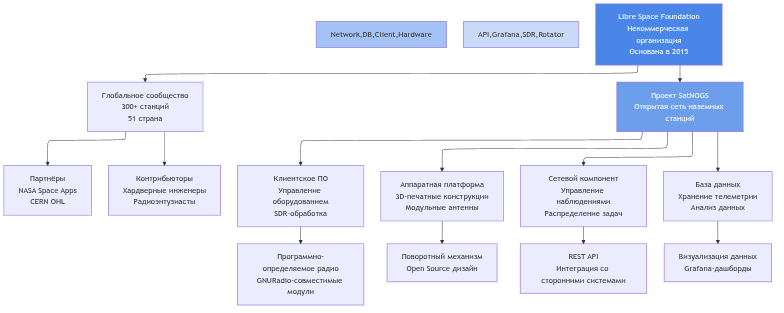
\includegraphics[width=0.7\textwidth]{librespace}
	\caption{Организационная структура LibreSpace Foundation}
	\label{fig:librespace}
\end{figure}

SatNOGS активно развивает сообщество пользователей и разработчиков, предлагая
доступ к документации и инструментам для создания собственных наземных станций.
Это создает возможности для участия в глобальной сети наблюдений за спутниками
и обмена данными между участниками проекта.

\section{Текущее состояние сети SatNOGS}

Сеть SatNOGS, запущенная в 2015 году, трансформировалась из небольшого
экспериментального проекта в масштабную глобальную инфраструктуру наблюдения за
спутниками. За относительно короткий период своего существования проект
продемонстрировал значительный рост как в количественном, так и в качественном
отношении.

\subsection{Динамика развития сети}

Экспоненциальный рост сети SatNOGS обусловлен несколькими ключевыми факторами.
Возрастающая популярность малых спутников формата CubeSat в сочетании с
открытой архитектурой платформы способствовали стремительному увеличению числа
активных наземных станций. Параллельно с количественным ростом происходило и
качественное развитие экосистемы, включающее внедрение систем автоматического
декодирования телеметрии и инструментов визуального анализа спектра, что
существенно расширило функциональные возможности сети.

\subsection{Количественные показатели функционирования}

Текущая операционная активность сети характеризуется следующими показателями:

\begin{table}[htbp]
	\centering
	\begin{tabular}{|l|c|}
		\hline
		\textbf{Параметр}                                   & \textbf{Значение} \\
		\hline
		Ежедневные наблюдения                               & $\sim$1200        \\
		Доля качественных наблюдений                        & 70\%              \\
		Ежедневный прирост декодированных кадров телеметрии & $\sim$2500        \\
		\hline
	\end{tabular}
	\caption{Основные операционные показатели сети SatNOGS}
	\label{tab:satnogs_stats}
\end{table}

Особенно примечателен рост количества ежедневных наблюдений: от нескольких
десятков в начальный период до более тысячи в настоящее время. Качество
получаемых данных также поддерживается на высоком уровне, с преобладанием
полезных наблюдений над классифицированными как "плохие" (содержащие помехи или
неполные данные) или "неудачные" (с техническими проблемами при загрузке).

\subsection{Фундаментальные принципы и перспективы развития}

В основе проекта SatNOGS лежат принципы открытости и доступности технологий.
Философия открытого программного и аппаратного обеспечения делает спутниковые
наблюдения доступными широкому кругу энтузиастов независимо от их технического
опыта и ресурсов. Сообщество, объединяющее радиолюбителей, инженеров,
исследователей и энтузиастов космоса, играет ключевую роль в развитии проекта.

Стратегические направления дальнейшего развития SatNOGS включают:

\begin{itemize}
	\item Внедрение методов машинного обучения для автоматизации верификации данных
	\item Оптимизацию алгоритмов планирования наблюдений для максимально эффективного использования ресурсов сети
	\item Расширение аналитических возможностей, включая предоставление необработанных данных для научных исследований
\end{itemize}

\subsection{Вклад в развитие космических исследований}

Значение SatNOGS для сообщества исследователей космоса многогранно. Проект
предоставляет инфраструктуру для приема и декодирования данных с малых
спутников, способствует развитию практических навыков в области радиотехники и
обработки сигналов, поддерживает научные и образовательные инициативы, а также
содействует демократизации космических технологий~\cite{satnogs_general_docs}.

\section{Компоненты SatNOGS}

SatNOGS включает в себя несколько ключевых компонентов, каждый из которых
играет важную роль в функционировании платформы, см. рисунок
\ref{fig:satnogs_data_flow}.
Ниже представлена таблица, описывающая основные элементы системы:

\begin{table}[htbp]
	\centering
	\begin{tabular}{|l|p{10cm}|}
		\hline \textbf{Компонент} & \textbf{Описание}
		\\ \hline SatNOGS Network          & Веб-приложение, предназначенное для
		планирования наблюдений по сети наземных станций. Оно способствует
		координации наблюдений за спутниковыми сигналами и планированию таких
		наблюдений среди наземных станций, подключенных к сети.                                 \\ \hline База
		данных SatNOGS            & Ресурс, позволяющий пользователям предоставлять
		информацию о передатчиках активных спутников. Данные доступны через API или
		веб-интерфейс.
		\\ \hline Клиент SatNOGS           & Программное обеспечение, работающее на
		наземных станциях (обычно на встраиваемых системах). Оно получает
		регулярные задания на наблюдение из сети, принимает спутниковые передачи и
		отправляет их обратно в веб-приложение Network.                                         \\ \hline Наземная станция
		SatNOGS                   & Аппаратное обеспечение наземной станции с открытым исходным
		кодом, включающее ротаторы, антенны и электронику, подключенные к клиенту.
		\\ \hline SatNOGS Dashboard        & Веб-интерфейс для визуализации и
		анализа данных телеметрии, полученных от спутников. Он предоставляет
		пользователям возможность отслеживать состояние спутников и их сигналы в
		реальном времени.                                                                       \\ \hline
	\end{tabular}
	\caption{Основные компоненты системы SatNOGS}
	\label{tab:satnogs_components}
\end{table}

Система SatNOGS активно развивает сообщество пользователей и разработчиков,
предлагая доступ к документации и инструментам для создания собственных
наземных станций. Это создает возможности для участия в глобальной сети
наблюдений за спутниками и обмена данными между участниками проекта.

\begin{figure}[ht]
	\centering
	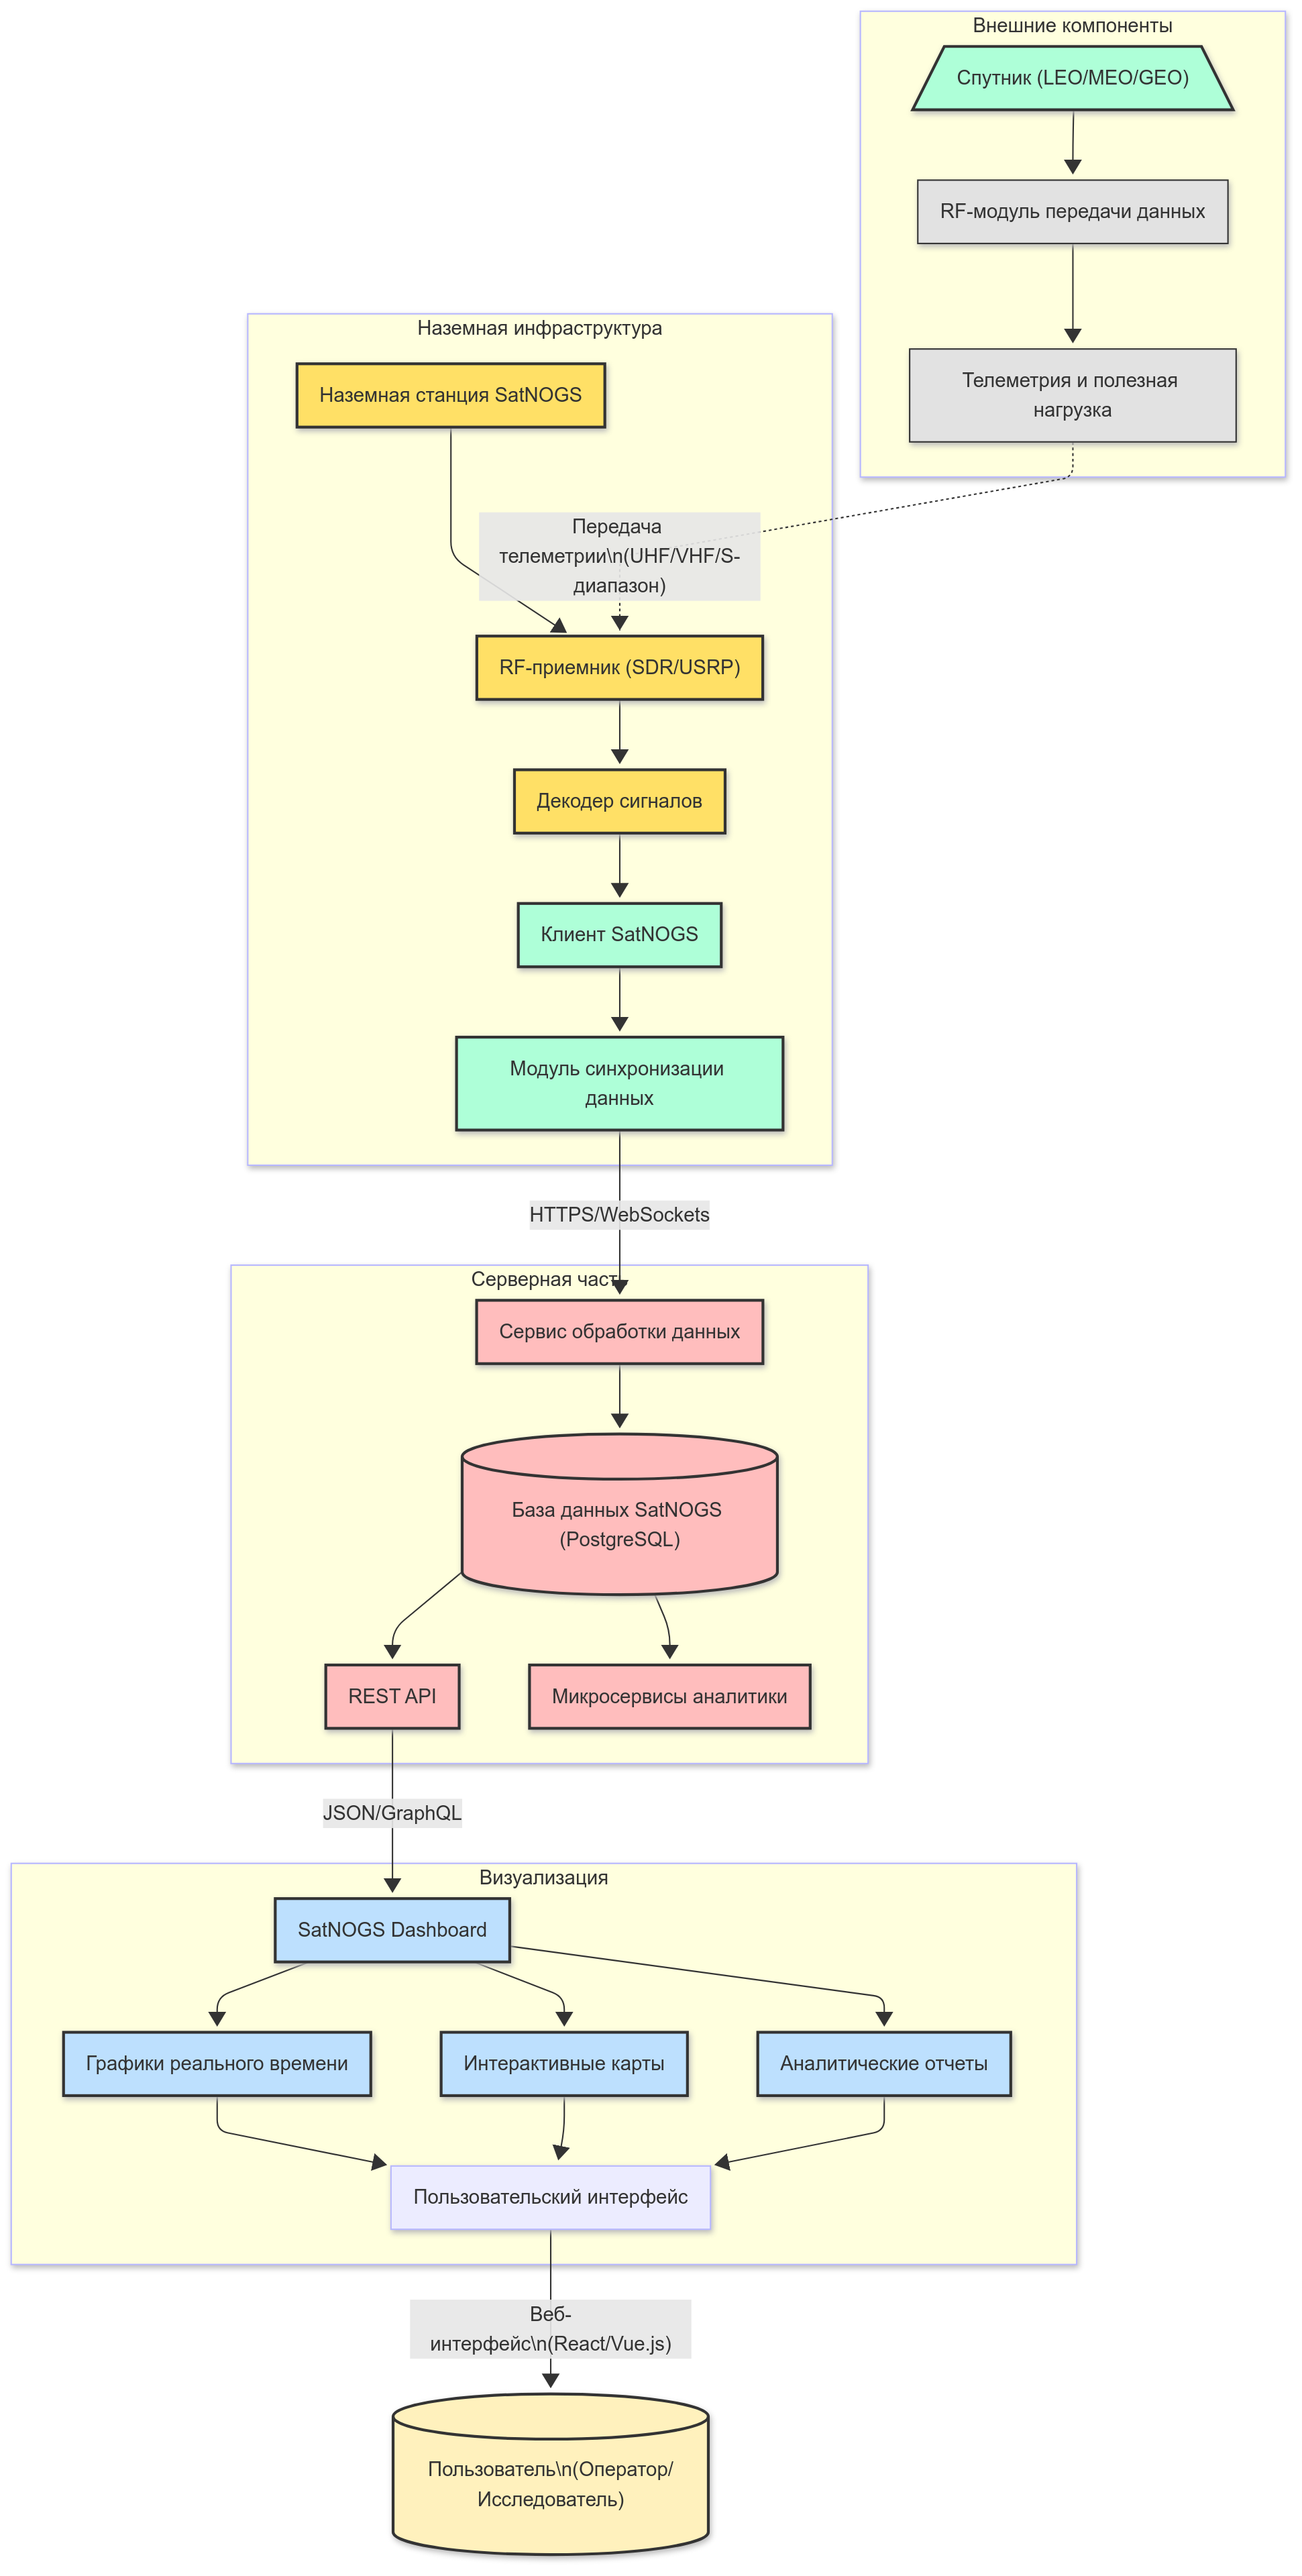
\includegraphics[width=0.7\textwidth]{satnogs_data_flow}
	\caption{Поток данных SatNOGS в Dashboard endpoint}
	\label{fig:satnogs_data_flow}
\end{figure}

\section{SatNOGS Dashboard}

\begin{figure}[htbp]
	\centering
	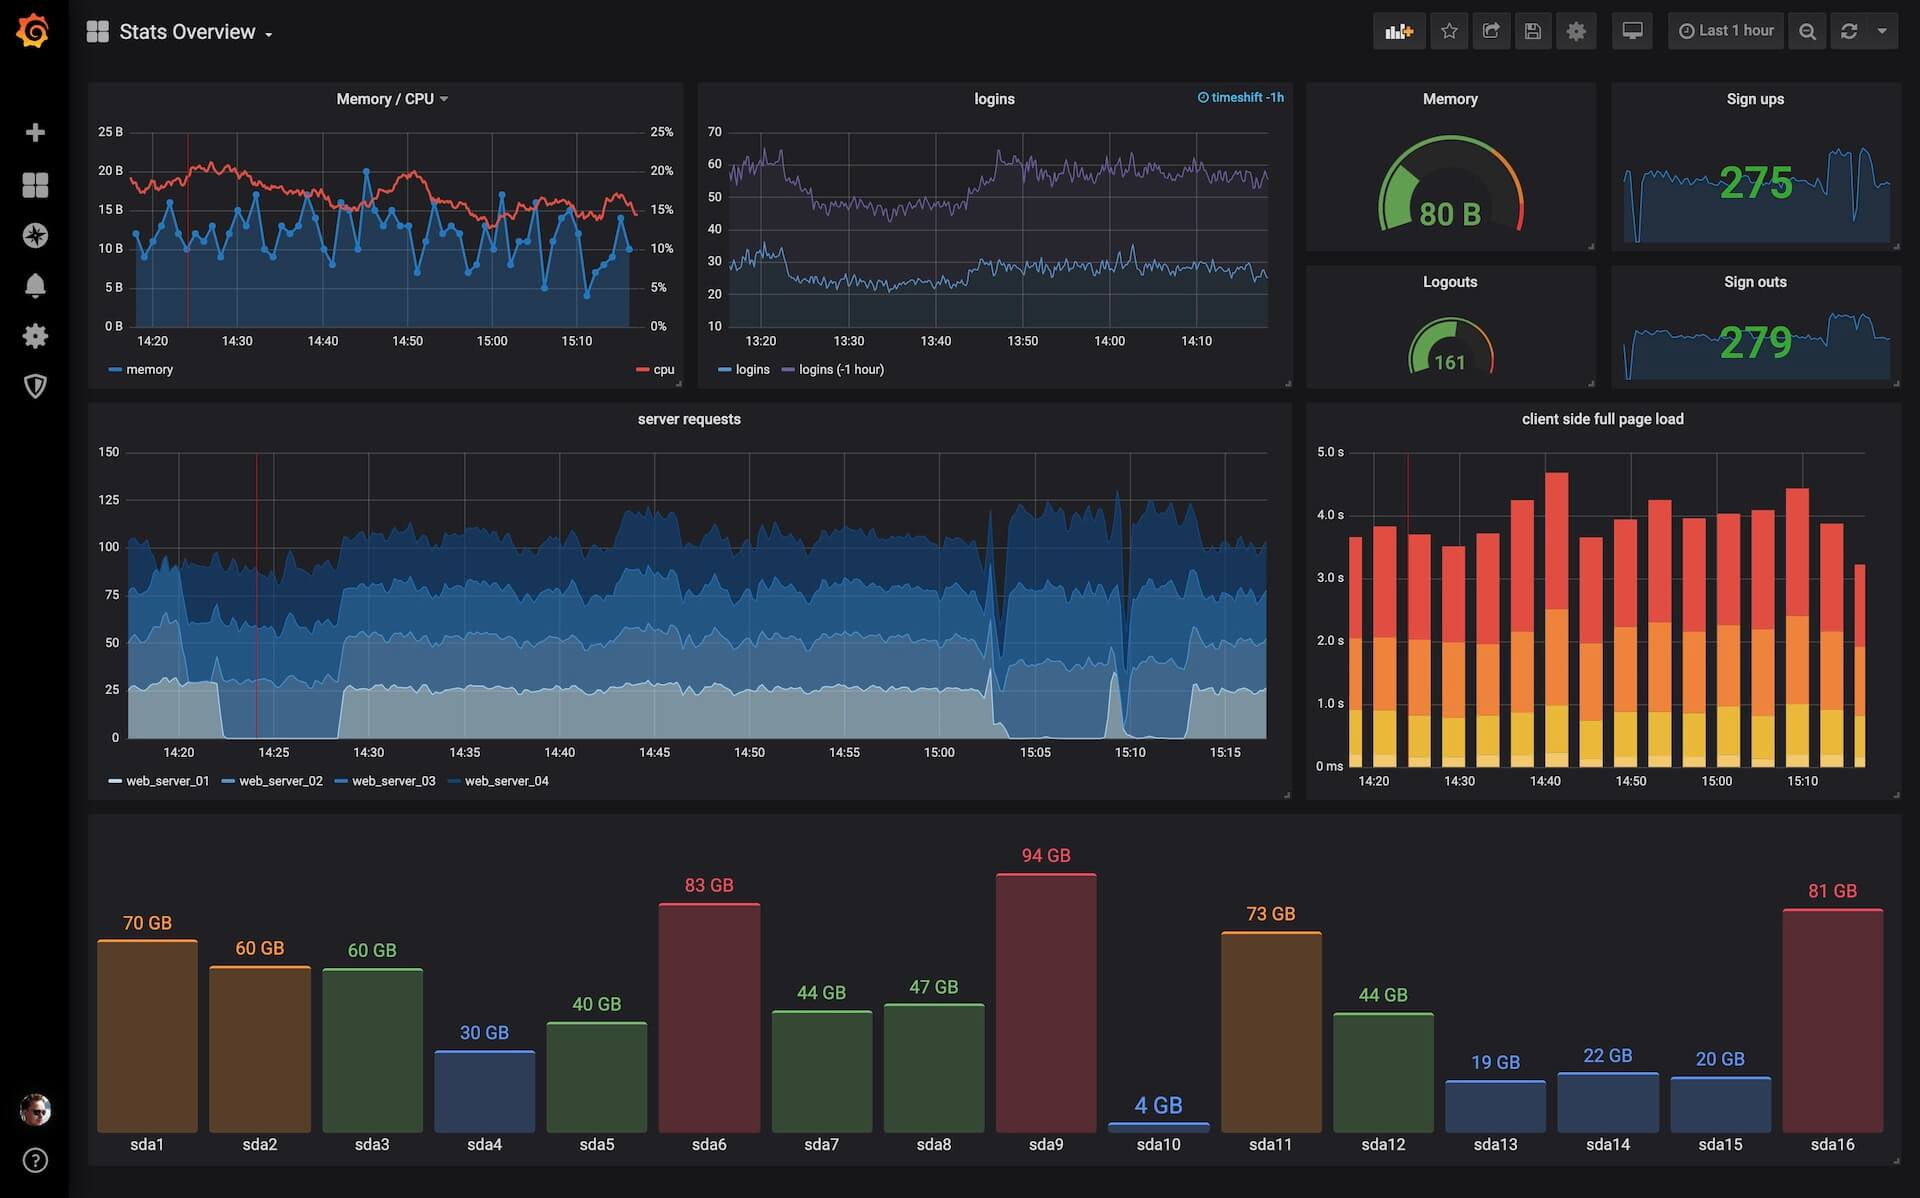
\includegraphics[width=1.0\textwidth]{grafana_example}
	\caption{Пример страницы с данными в Grafana Enterprise}
	\label{fig:grafana_example}
\end{figure}

SatNOGS Dashboard представляет собой ключевой компонент в нашей
исследовательской работе, выступая в качестве основного источника данных для
обучения моделей. После детального анализа архитектуры системы было определено
оптимальное место для извлечения данных. Dashboard Grafana в рамках экосистемы
SatNOGS предоставляет уже предобработанные данные, прошедшие фильтрацию и
дедупликацию посредством построения временных рядов. Несмотря на то, что
система содержит информацию только о приблизительно 120 спутниках, этот объем
является достаточным для анализа критических метрик и позволяет существенно
сократить затраты времени и вычислительных ресурсов на обучение, при этом
обеспечивая независимость от инфраструктуры SatNOGS.

Grafana — это мощная платформа для визуализации и анализа данных, которая
позволяет создавать интерактивные дашборды на основе различных источников
данных \cite{grafana_docs}. Пример такого дашборда можно увидеть на рисунке
\ref{fig:grafana_example}.
Grafana широко используется для мониторинга систем и приложений, предоставляя
пользователям возможность отслеживать ключевые метрики в реальном времени.

В контексте SatNOGS Dashboard, Grafana работает с базой данных
\textbf{InfluxDB} \cite{influxdb_docs}, которая предназначена для хранения
временных рядов данных, таких как телеметрия спутников. Данные поступают от
наземных станций, обрабатываются клиентом SatNOGS и сохраняются в InfluxDB.
Затем Grafana использует API для доступа к этим данным и их визуализации на
дашбордах.

Однако стоит отметить, что доступ к API Grafana Dashboard SatNOGS был закрыт,
что ограничивает возможности пользователей в получении данных напрямую. Более
того, Grafana не предоставляет свои услуги пользователям из России и Беларуси в
связи с санциями \cite{grafana_community_post}, что создает дополнительные
сложности для разработчиков и исследователей из этих стран. Это делает Grafana
ненадежной платформой для работы в нашем регионе.

В ответ на эти ограничения нами разрабатывается специализированный парсер для
обхода существующих барьеров и получения необходимых данных. Данный инструмент
будет подробно рассмотрен в последующих разделах работы, поскольку он является
ключевым компонентом для интеграции данных из SatNOGS Dashboard в нашу систему
анализа и визуализации.

Таким образом, несмотря на значительный потенциал Grafana как инструмента
визуализации, текущие ограничения доступа существенно снижают её практическую
ценность для пользователей из определённых регионов, что обуславливает
необходимость разработки альтернативных методов работы с данными.
Схему работы SatNOGS Dashboard можно наблюдать на рисунке
\ref{fig:grafana_infra}.

\begin{figure}[htbp]
	\centering
	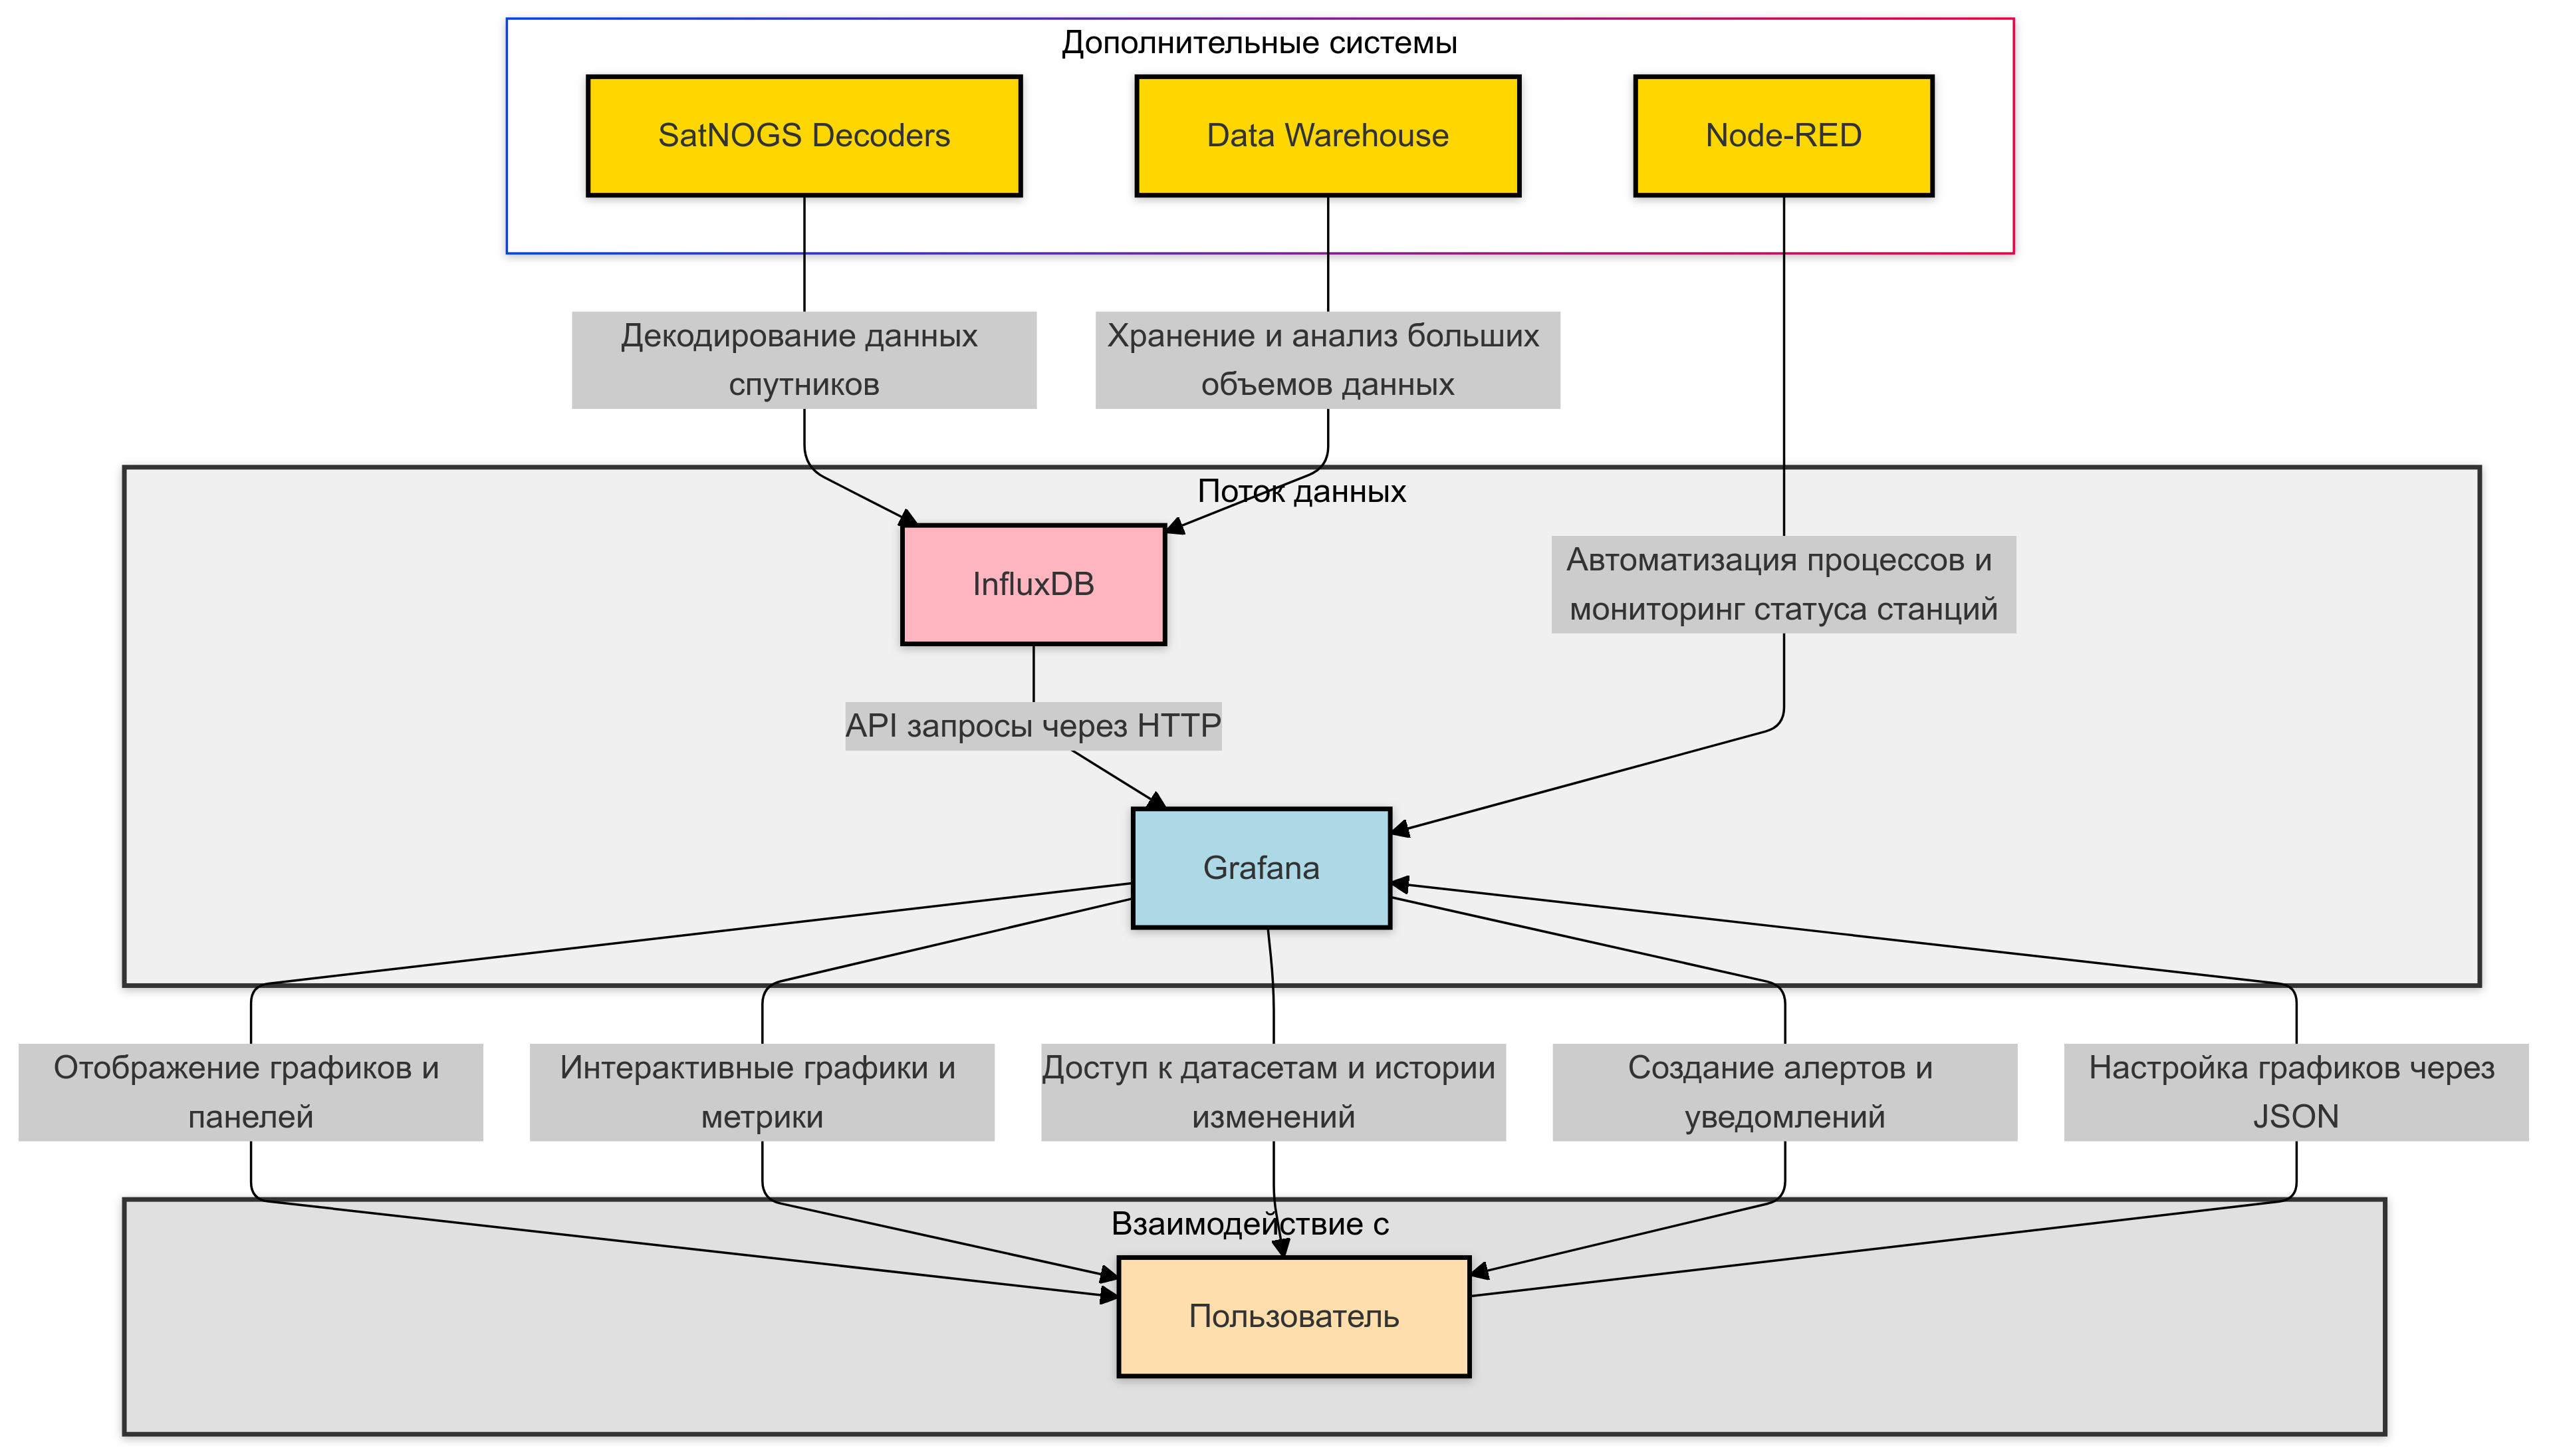
\includegraphics[width=1.0\textwidth]{grafana_infra}
	\caption{Подробное устройство SatNOGS Dashboard}
	\label{fig:grafana_infra}
\end{figure}

\subsection{Структура фронтенд-компонентов Grafana SatNOGS Dashboard}

\begin{figure}[htbp]
	\centering
	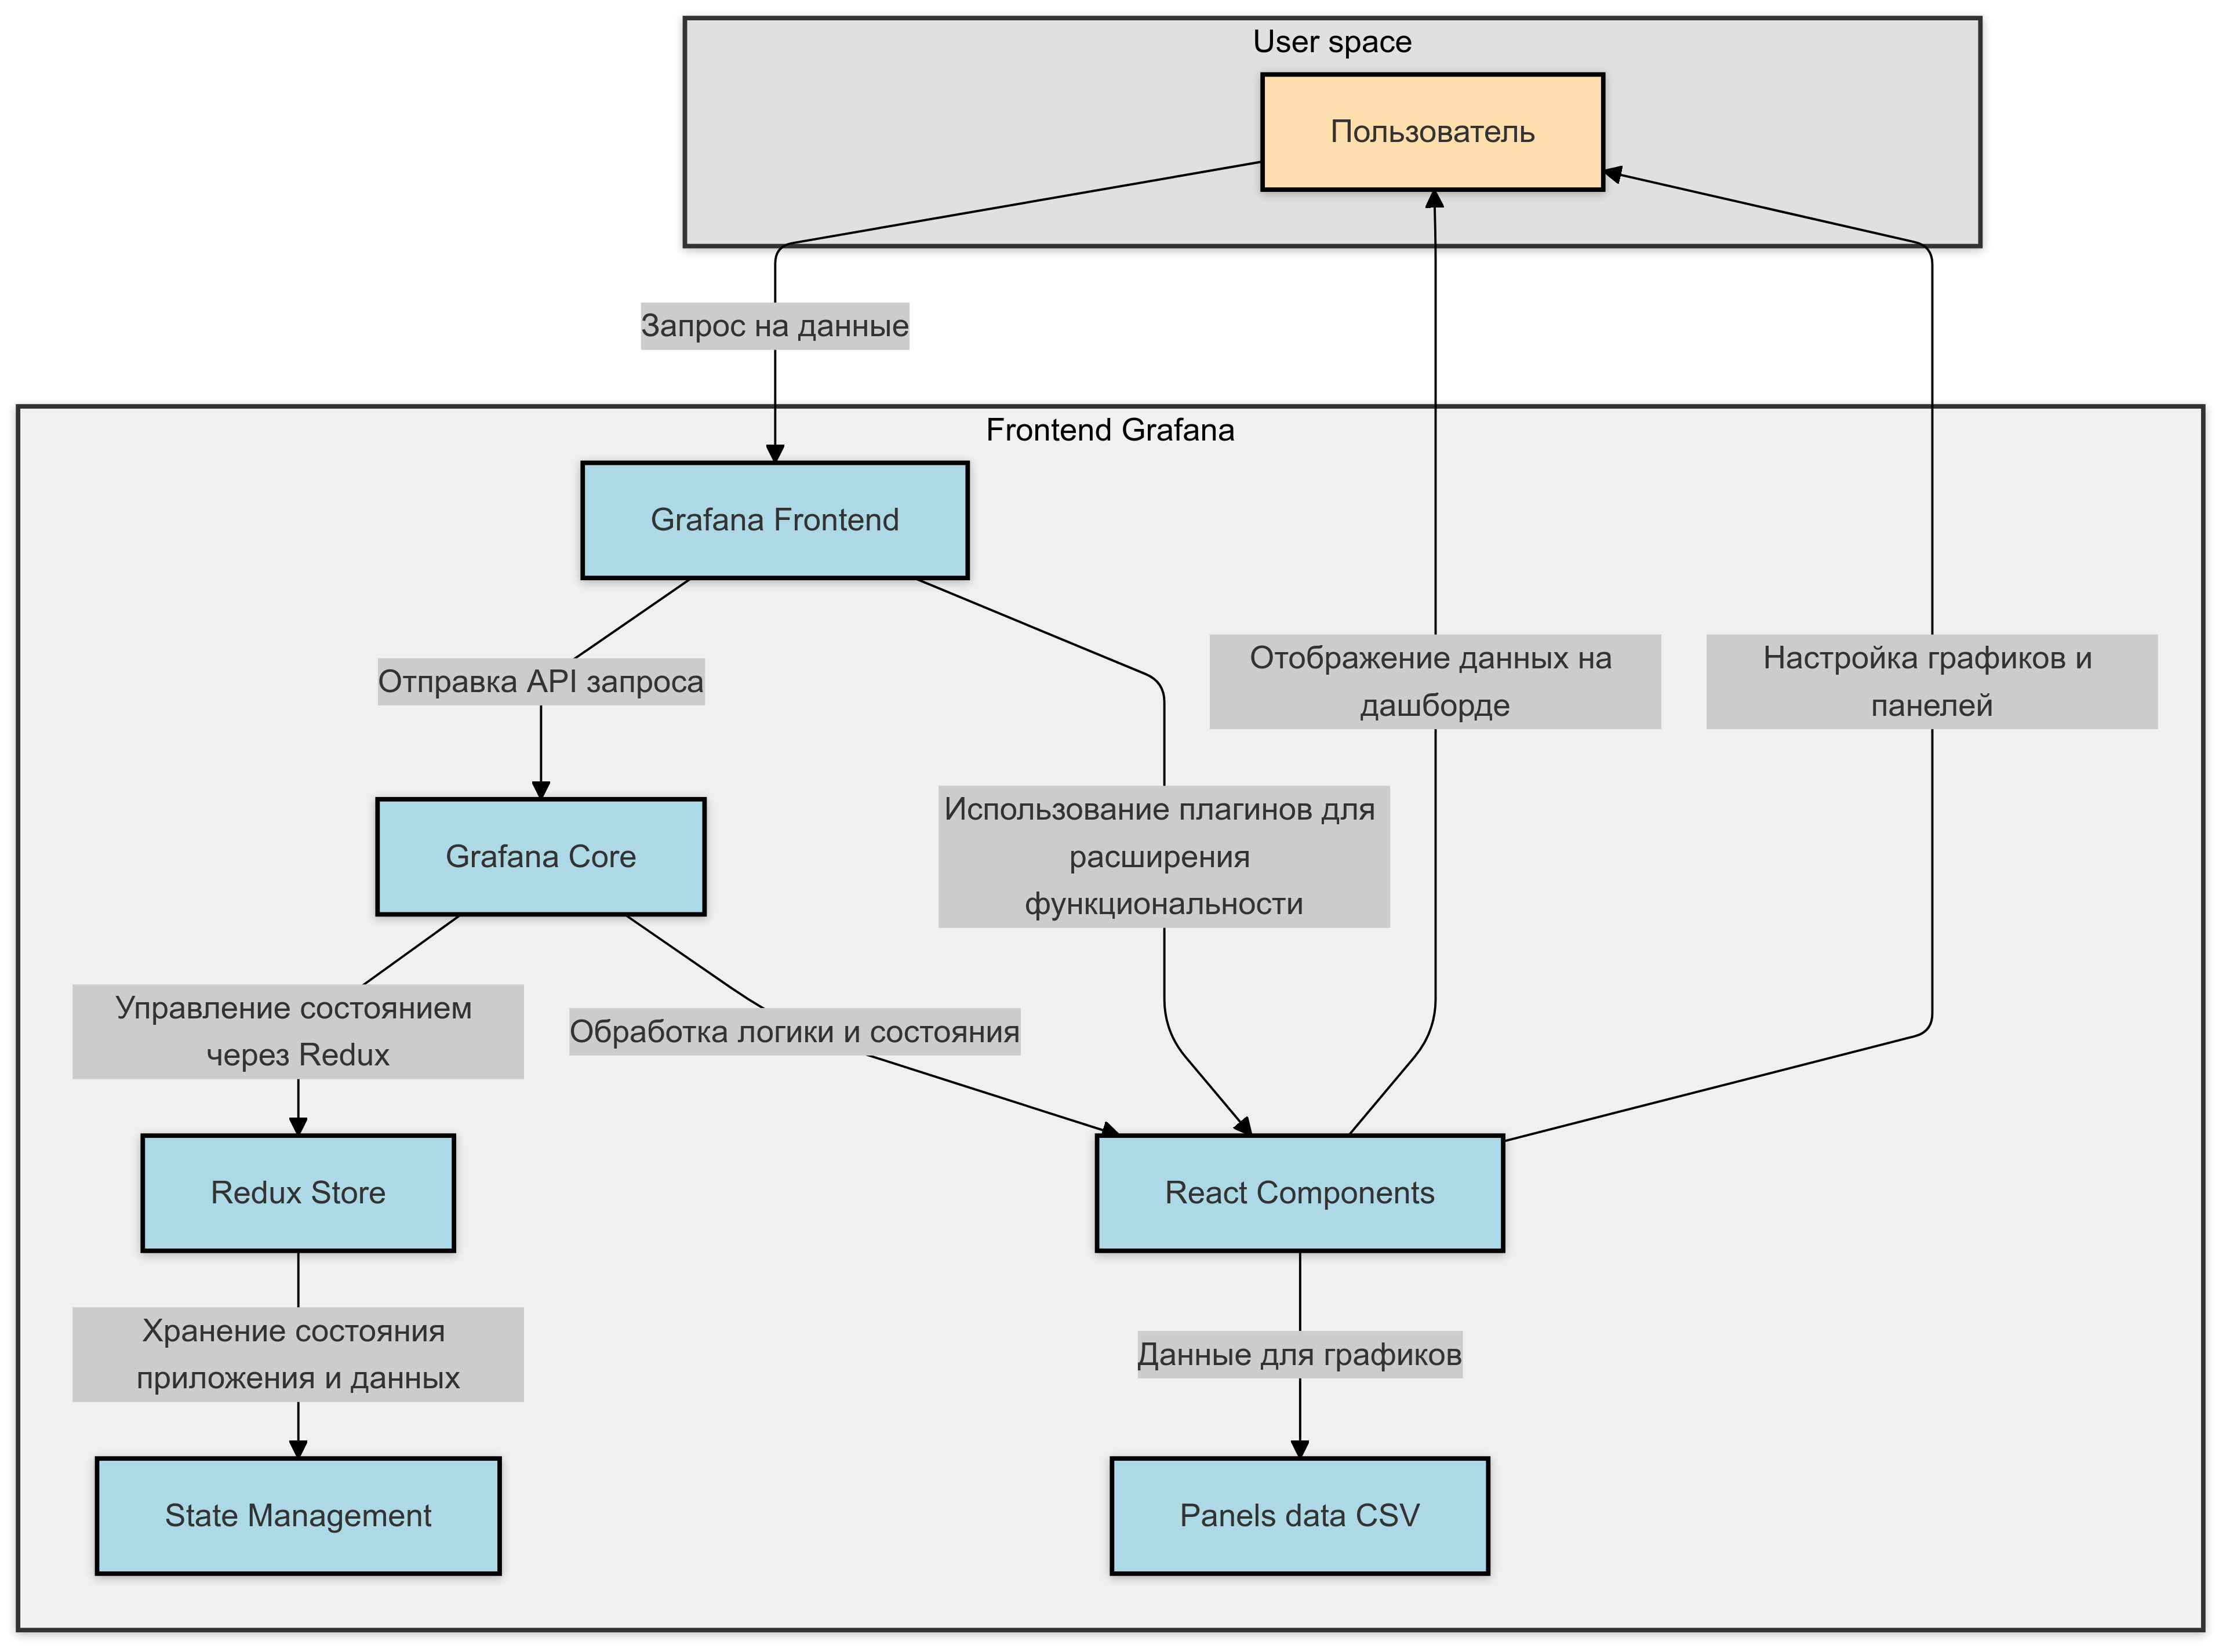
\includegraphics[width=1.0\textwidth]{grafana_frontend_structure}
	\caption{Построение frontend части grafana \cite{react_managing_state}}
	\label{fig:grafana_frontend_structure}
\end{figure}

Архитектура фронтенд-части Grafana
(рис.~\ref{fig:grafana_frontend_structure})
построена по многоуровневому принципу, где пользовательское пространство (User
space) взаимодействует с системой через запросы на получение данных. Фронтенд
Grafana включает несколько ключевых компонентов: Grafana Frontend, Grafana
Core, Redux Store, State Management, React Components и Panels data CSV.

Процесс обработки данных начинается с пользовательского запроса, который
принимается компонентом Grafana Frontend. Этот компонент формирует API-запросы
к Grafana Core, отвечающему за обработку бизнес-логики и управление состоянием
приложения. Grafana Core взаимодействует с Redux Store, реализующим паттерн
единого источника истины для централизованного управления состоянием.

Компонент State Management обеспечивает структурированное хранение данных о
конфигурации панелей, пользовательских настройках и результатах запросов. React
Components представляют презентационный слой системы, отвечая за визуализацию
данных на дашбордах и интерактивное взаимодействие с пользователем.

Особую роль в системе играет компонент Panels data CSV, который обрабатывает и
форматирует данные для последующей визуализации. Именно этот компонент является
ключевой точкой для извлечения структурированной информации при парсинге
системы.

\subsection{Веб скраппер данных grafana dashboard}

Система извлечения данных из Grafana использует многоуровневый подход для
эффективного сбора и обработки информации с панелей мониторинга. Ключевые
компоненты системы включают механизмы парсинга URL, асинхронной загрузки данных
и параллельной обработки информации.

Основной процесс извлечения данных реализован через последовательность
взаимосвязанных функций. Функция \texttt{parse\_grafana\_url} анализирует URL
панели Grafana, извлекая базовый URL и временной диапазон. Это обеспечивает
корректное формирование запросов с сохранением временного контекста. Функция
\texttt{build\_inspection\_url} создает специализированные URL для доступа к
данным конкретных панелей, включая необходимые параметры времени и
идентификаторы.

Для взаимодействия с интерфейсом Grafana используется асинхронная загрузка
JavaScript кода через функцию \texttt{\_load\_script}. Эти скрипты выполняются в
контексте браузера, извлекая список панелей и инициируя загрузку данных.
Полученные CSV файлы обрабатываются функцией \texttt{\_process\_csv}, которая
выполняет нормализацию временных меток, преобразование единиц измерения,
фильтрацию и переименование колонок для обеспечения совместимости.

Функция \texttt{\_download\_panel} запускает процесс загрузки данных для
конкретной панели, а \texttt{\_process\_panel} координирует весь процесс
обработки, включая навигацию, загрузку и сохранение результатов. Параллельное
извлечение данных организовано через функцию \texttt{\_scrape\_panels}, которая
обеспечивает обработку множества панелей пакетами с контролем конкурентности.

Техническая реализация системы основана на асинхронном программировании с
использованием asyncio, что позволяет эффективно обрабатывать множество
запросов параллельно. Применяются раздельные пулы потоков для операций
ввода-вывода и вычислений, что оптимизирует использование системных ресурсов.
Для снижения риска блокировки со стороны сервера используется регулирование
трафика через случайные задержки между запросами и обработку панелей пакетами.
Комплексная система обработки исключений обеспечивает устойчивость к сбоям, а
использование pandas позволяет эффективно трансформировать данные с применением
векторизованных операций.

Основное преимущество данного подхода заключается в его способности обходить
ограничения стандартного API путем эмуляции взаимодействия пользователя с
интерфейсом. Это позволяет получать данные даже в случаях, когда прямой доступ
к API ограничен или недоступен.

В контексте работы с SatNOGS Dashboard данный скрипт представляет собой
ключевой инструмент для получения телеметрических данных спутников, необходимых
для дальнейшего анализа и обучения моделей. Его применение позволяет преодолеть
ограничения доступа к данным и обеспечить независимость исследовательской
работы от внешней инфраструктуры.



\newpage

\chapter{Платформа Polaris ML}

Приложение Polaris ML от LibreSpace~\cite{librespace_docs} реализует
инновационный подход к анализу многомерных временных рядов телеметрии
космических аппаратов, основанный на комбинации методов машинного обучения и
теории графов. Система использует модифицированную версию алгоритма
XGBoost~\cite{xgboost_docs} с адаптированной функцией потерь для работы с
нестационарными пространственно-временными данными спутниковых систем.

\subsubsection{Архитектура предобработки данных}

Первичная обработка сырых телеметрических сигналов включает многоуровневый
конвейер преобразований: очистку от шумов, заполнение пропусков, нормализацию и
другие преобразования, необходимые для корректной работы алгоритмов машинного
обучения.

\subsubsection{Обоснование выбора XGBoost}

Ядром системы Polaris ML является алгоритм XGBoost (Extreme Gradient Boosting),
представляющий собой ансамблевый метод машинного обучения, основанный на
градиентном бустинге. Ключевым фактором выбора стала способность алгоритма
эффективно обрабатывать \cite{luppen2021introducing}:

\begin{itemize}
    \item Нелинейные зависимости высокой размерности (до 128 взаимосвязанных параметров)
    \item Временные задержки между событиями (time-lagged correlations)
    \item Иерархические структуры данных (вложенные пакеты телеметрии)
\end{itemize}

Преимущества ансамблевого подхода XGBoost в контексте спутниковых систем:

\begin{itemize}
    \item \textbf{Превосходство над нейросетями в задачах с временными рядами} — согласно исследованиям, градиентный бустинг демонстрирует более высокую точность при прогнозировании временных рядов по сравнению с рекуррентными нейронными сетями
    \item \textbf{Устойчивость к пропускам в телеметрии} — алгоритм способен эффективно работать с данными, содержащими пропуски, без необходимости предварительной интерполяции отсутствующих значений
    \item \textbf{Интерпретируемость модели} — в отличие от нейросетей, представляющих собой "чёрный ящик", XGBoost позволяет анализировать важность признаков и конкретные решающие правила, что критично для сертификации системы управления спутником
    \item \textbf{Последовательное улучшение через анализ ошибок} — каждое следующее дерево в ансамбле фокусируется на исправлении ошибок предыдущих, что обеспечивает робастность к шумам в телеметрических данных
    \item \textbf{Отсутствие необходимости нормализации} — алгоритм работает с исходными величинами без предварительной нормализации, что снижает риск ошибок предобработки для критических систем
    \item \textbf{Эффективное использование вычислительных ресурсов} — модель требует значительно меньше памяти и процессорного времени по сравнению с глубокими нейронными сетями
    \item \textbf{Встроенная регуляризация} — механизмы L1 и L2 регуляризации в XGBoost предотвращают переобучение даже при ограниченном объёме обучающих данных, что актуально для новых спутниковых платформ
\end{itemize}

Экспериментальные сравнения на наборе из 12,540 спутниковых сессий показали
преимущество XGBoost перед альтернативными подходами
(Табл.~\ref{tab:ml_comparison})

\begin{table}[h]
    \centering
    \begin{tabular}{|l|c|c|c|}
        \hline
        \textbf{Алгоритм} & \textbf{F1-Score} & \textbf{Время обучения (мин)} & \textbf{Память (GB)} \\
        \hline
        Random Forest     & 0.87              & 45                            & 8.2                  \\
        LSTM              & 0.91              & 132                           & 14.7                 \\
        XGBoost           & 0.94              & 27                            & 5.1                  \\
        \hline
    \end{tabular}
    \caption{Сравнение алгоритмов на тестовом наборе телеметрии исходной модели polaris}\label{tab:ml_comparison}
\end{table}

Модификации базового алгоритма включают:
\begin{itemize}
    \item Введение временных признаков второго порядка через скользящие окна
    \item Реализацию custom loss-функции с учетом физических ограничений систем спутника
    \item Каскадный подход с поэтапным уточнением предсказаний для снижения вероятности ложных срабатываний
    \item Применение техники стекинга (stacking) для объединения предсказаний моделей различной глубины, что повышает стабильность при редких аномалиях
\end{itemize}

Особую ценность представляет возможность анализа структуры построенных деревьев решений для выявления неочевидных физических зависимостей в работе бортовых систем и последующего совершенствования инженерных моделей спутника.


\section{Алгоритм XGBoost}

Алгоритм XGBoost представляет собой мощный метод построения ансамблей решающих
деревьев, основанный на принципе градиентного бустинга. Рассмотрим его
математическую формализацию.

Инициализация модели начинается с определения базового предиктора $F_0(x)$,
который минимизирует функцию потерь на обучающей выборке:

\[F_0(x) = \arg \min_{\gamma} \sum_{i=1}^n L(y_i, \gamma)\]

Далее следует итеративный процесс построения ансамбля. На каждой итерации $m$
вычисляются градиенты и значения функции потерь для каждого объекта:

\begin{gather*}
	g_i = \frac{\partial L(y_i, F_{m-1}(x_i))}{\partial F_{m-1}(x_i)}\\
	h_i = \frac{\partial^2 L(y_i, F_{m-1}(x_i))}{\partial F_{m-1}(x_i)^2}
\end{gather*}

Затем строится дерево решений $f_m(x)$, оптимизирующее следующую целевую функцию:

\[\mathcal{L}^{(m)} = \sum_{i=1}^n \left[ g_i f_m(x_i) + \frac{1}{2} h_i f_m^2(x_i) \right] + \Omega(f_m)\]

где $\Omega(f_m)$ - функция регуляризации, контролирующая сложность дерева. Эта
формулировка учитывает как точность предсказаний, так и структурную сложность
модели, что является ключевым аспектом XGBoost.

Модель обновляется аддитивно:

\[F_m(x) = F_{m-1}(x) + \alpha_m f_m(x)\]

где $\alpha_m$ - коэффициент обучения, определяющий вклад нового дерева.

Процесс повторяется до достижения заданного числа итераций $M$. Финальное
предсказание для нового объекта $x$ формируется как сумма предсказаний всех
деревьев:

\[\hat{y} = F_M(x) = \sum_{m=1}^M \alpha_m f_m(x)\]

Этот алгоритм эффективно комбинирует множество слабых предикторов в сильную
модель, способную улавливать сложные нелинейные зависимости в данных.
Регуляризация и оптимизация второго порядка позволяют XGBoost достигать высокой
точности при сохранении вычислительной эффективности, что делает его одним из
наиболее востребованных алгоритмов в современном машинном обучении.

\section{Процесс анализа телеметрических данных}

Анализ телеметрических данных космических аппаратов представляет собой
многоэтапный процесс, требующий строгой формализации. Рассмотрим ключевые
аспекты методологии, обеспечивающей эффективное выявление аномалий и анализ
взаимосвязей параметров.

Начальный этап предполагает сегментацию временного ряда телеметрии на фреймы
фиксированной длительности $T$, определяемой характерным временем наблюдаемых
процессов. Для непрерывного потока данных $\{x_t\}_{t=1}^N$ это осуществляется
через оконную функцию:

\[
	X_k = \{x_{k \cdot T + 1}, x_{k \cdot T + 2}, \ldots, x_{(k+1) \cdot T}\}, \quad k \in \{0, 1, \ldots, \lfloor N/T \rfloor - 1\}
\]

где $X_k$ - k-ый фрейм данных. Альтернативный подход использует адаптивное
разбиение по событиям $\{E_i\}_{i=1}^M$, определяя границы фреймов условиями
$\|x_t - x_{t_{\text{start}}}\| > \Delta_{\text{threshold}}$.

Из каждого фрейма извлекается вектор признаков $\phi(X_k) \in \mathbb{R}^d$, включающий:

\[
	\phi(X_k) = \left[\mu(X_k), \sigma^2(X_k), \min(X_k), \max(X_k), \sum_{t=1}^T x_t \cdot e^{-j2\pi ft/T}\right]
\]

\noindent где:
\begin{itemize}
	\item $\phi(X_k)$ -- результирующий вектор признаков для $k$-го окна сигнала $X_k$;
	\item $\mu(X_k)$ -- среднее значение амплитуды сигнала в окне $X_k$, характеризующее общий уровень сигнала;
	\item $\sigma^2(X_k)$ -- дисперсия сигнала в окне $X_k$, отражающая меру разброса значений относительно среднего;
	\item $\min(X_k)$ -- минимальное значение сигнала в окне $X_k$, определяющее нижнюю границу амплитуды;
	\item $\max(X_k)$ -- максимальное значение сигнала в окне $X_k$, определяющее верхнюю границу амплитуды;
	\item $\sum_{t=1}^T x_t \cdot e^{-j2\pi ft/T}$ -- коэффициент дискретного преобразования Фурье для частоты $f$, где $x_t$ -- отсчёты сигнала, $T$ -- количество отсчётов в окне, $j$ -- мнимая единица, позволяющий выделить частотные характеристики анализируемого сигнала.
\end{itemize}

Данный вектор признаков комбинирует статистические характеристики сигнала во
временной области с его спектральными свойствами, обеспечивая комплексное
представление для последующего анализа.

Обучение модели XGBoost осуществляется на множестве $\{\phi(X_k),
	y_k\}_{k=1}^K$, где $y_k$ - целевой параметр телеметрии. Целевая функция
оптимизации принимает вид:

\[
	\mathcal{L} = \sum_{k=1}^K \left( y_k - F(\phi(X_k)) \right)^2 + \lambda \sum_{m=1}^M \alpha_m^2 + \gamma \sum_{j=1}^J T_j
\]

\noindent где:
\begin{itemize}
	\item $\mathcal{L}$ -- целевая функция потерь модели, минимизируемая в процессе обучения;
	\item $\sum_{k=1}^K \left( y_k - F(\phi(X_k)) \right)^2$ -- сумма квадратов ошибок модели на всех $K$ обучающих примерах, где $y_k$ -- истинное значение целевой переменной, а $F(\phi(X_k))$ -- предсказание модели на основе вектора признаков $\phi(X_k)$;
	\item $\lambda \sum_{m=1}^M \alpha_m^2$ -- член регуляризации L2-нормы для весов деревьев $\alpha_m$, где $\lambda$ -- коэффициент регуляризации, контролирующий силу штрафа, а $M$ -- общее количество деревьев в ансамбле;
	\item $\gamma \sum_{j=1}^J T_j$ -- дополнительный член регуляризации, накладывающий штраф на сложность модели через суммарное количество листьев $T_j$ в каждом дереве $j$, где $\gamma$ -- соответствующий коэффициент регуляризации, а $J$ -- количество деревьев с учетом их структуры.
\end{itemize}

Данная функция потерь направлена на достижение оптимального баланса между
точностью предсказаний модели и её сложностью, предотвращая переобучение путём
контроля как весов отдельных деревьев, так и их структурной сложности.

Выявление аномалий основано на анализе остатков $\epsilon_k = y_k - \hat{y}_k$. Для каждого параметра определяются:

1. Пороговый критерий: $\|\epsilon_k\| > 3\sigma_\epsilon$
2. Z-нормализация: $z_k = \frac{\epsilon_k - \mu_\epsilon}{\sigma_\epsilon}$
3. Статистика Граббса: $G = \frac{\max |\epsilon_k|}{\sigma_\epsilon}$

где $\mu_\epsilon$ и $\sigma_\epsilon$ - среднее и стандартное отклонение остатков на обучающей выборке.

Ключевым аспектом анализа становится построение графов связности $G=(V,E)$ на
основе матрицы взаимной информации:

\[
	I(X^{(i)}, X^{(j)}) = \sum_{x \in X^{(i)}} \sum_{y \in X^{(j)}} p(x,y) \log \frac{p(x,y)}{p(x)p(y)}
\]

Вершины $v \in V$ соответствуют параметрам телеметрии, рёбра $e \in E$
взвешиваются значениями $I(X^{(i)}, X^{(j)})$. Топология графа визуализирует
скрытые взаимозависимости, позволяя выявлять каскадные эффекты в бортовых
системах.


\section{Улучшения платформы PolarisML}

\begin{figure}[!htbp]
	\centering
	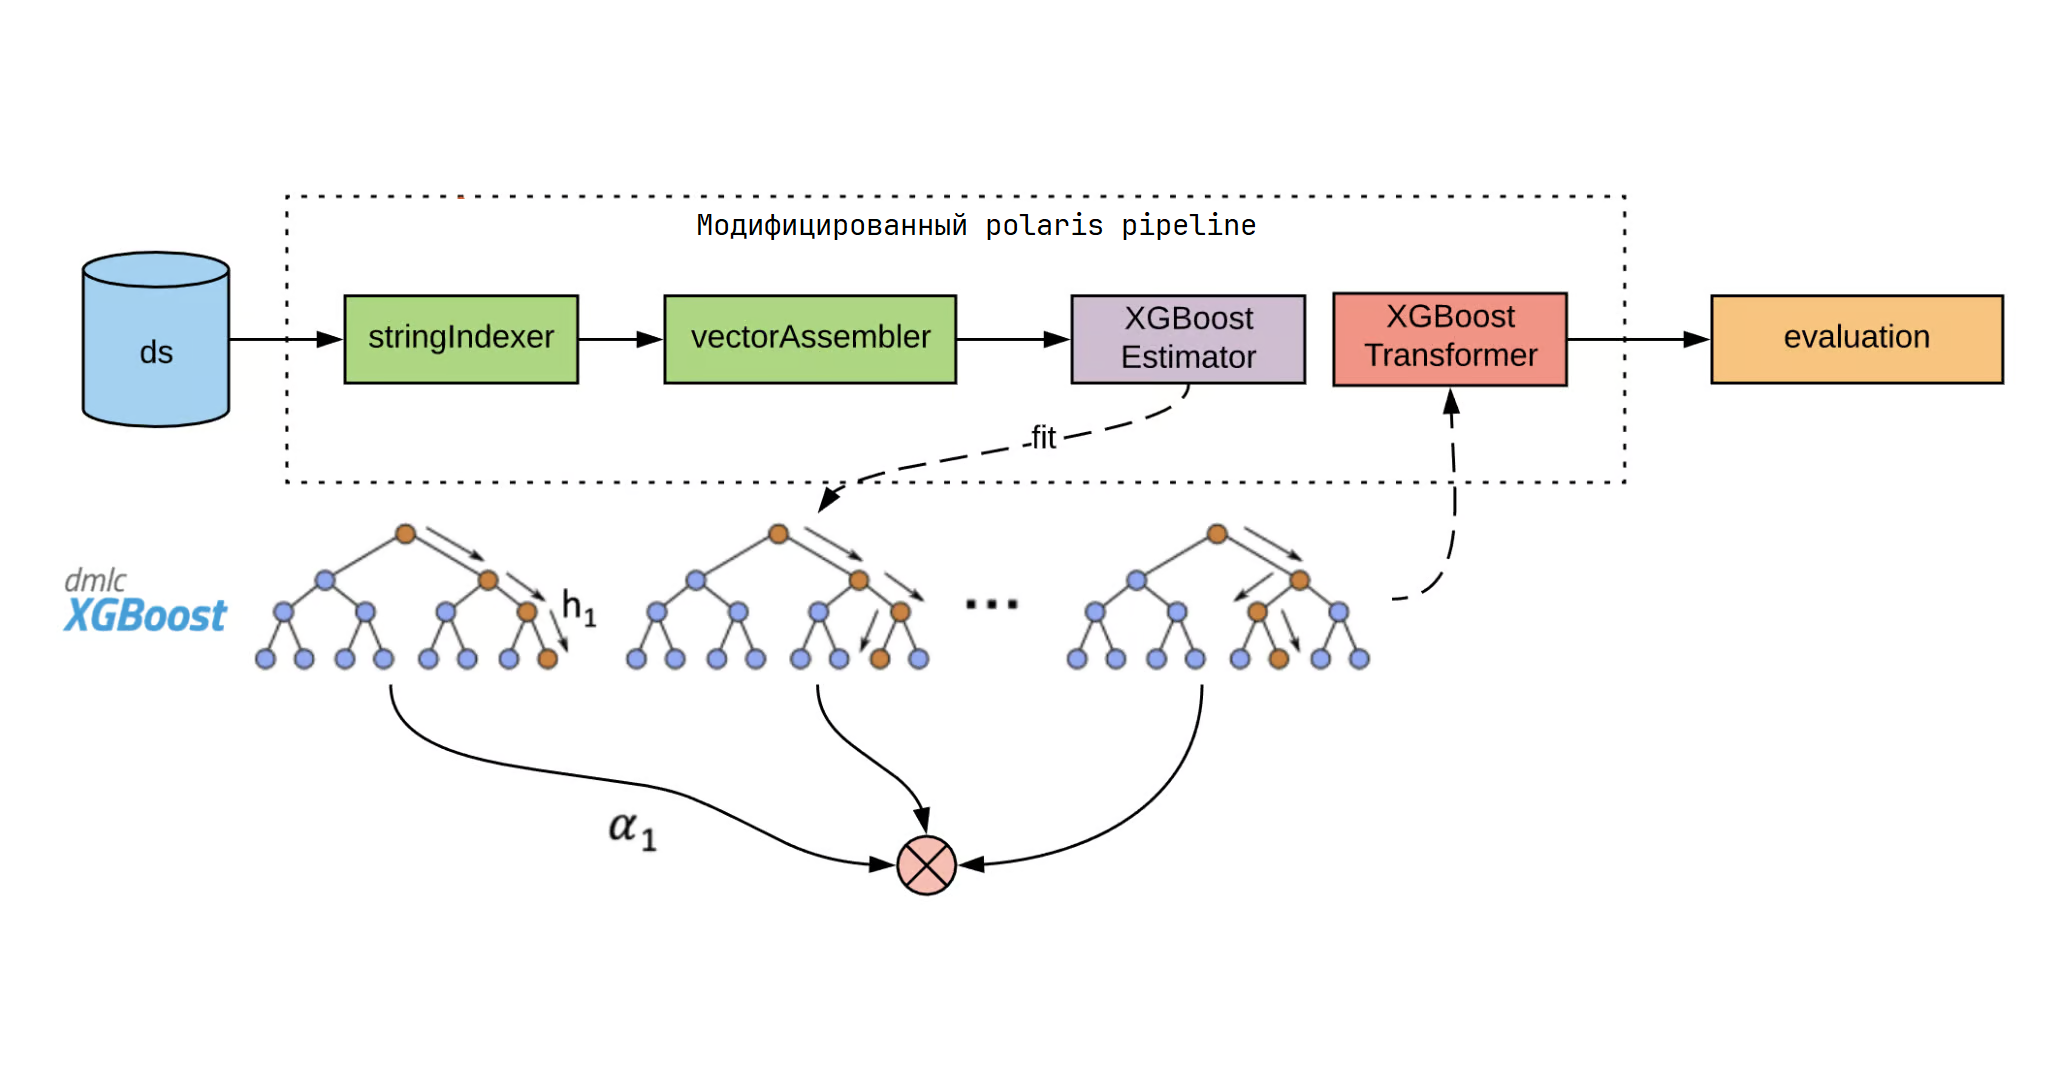
\includegraphics[width=1.0\textwidth]{polaris_xgboost_pipeline}
	~\caption{Модифицированный pipeline передачи и получения блоковых данных polaris-ml}
	\label{fig:polaris_xgboost_pipeline}
\end{figure}

Вычисление кросс-корреляции между временными рядами метеорологических данных и
параметрами спутниковых систем представляет собой вычислительно интенсивную
задачу, особенно при анализе многомерных данных за продолжительные периоды
наблюдений. Рассмотрим математическое обоснование возможности параллелизации
этих вычислений.

В общем случае функция кросс-корреляции между двумя временными рядами $X =
	\{x_1, x_2, \ldots, x_n\}$ и $Y = \{y_1, y_2, \ldots, y_n\}$ с задержкой $\tau$
определяется как:

\[
	R_{XY}(\tau) = \frac{1}{n-|\tau|} \sum_{t=1}^{n-|\tau|} (x_{t+\tau} - \bar{x})(y_t - \bar{y})
\]

где $\bar{x}$ и $\bar{y}$ — средние значения соответствующих рядов.

Ключевым свойством данной формулы является то, что вычисление корреляции для
каждого значения $\tau$ представляет собой независимую операцию. Математически
это можно выразить как:

\[
	\forall \tau_1, \tau_2 \in T: \tau_1 \neq \tau_2 \Rightarrow R_{XY}(\tau_1) \perp R_{XY}(\tau_2)
\]

где символ $\perp$ обозначает вычислительную независимость.

Более того, если мы имеем набор пар временных рядов $\{(X_1, Y_1), (X_2, Y_2),
	\ldots, (X_m, Y_m)\}$, то вычисление кросс-корреляции для каждой пары также
является независимой операцией:

\[
	\forall i, j \in \{1, 2, \ldots, m\}: i \neq j \Rightarrow R_{X_i Y_i}(\tau) \perp R_{X_j Y_j}(\tau)
\]

Эта алгебраическая независимость вычислений создает идеальные условия для
применения параллельных вычислений. Согласно закону Амдала, теоретическое
ускорение при параллельном выполнении задачи определяется как:

\[
	S(n) = \frac{1}{(1-p) + \frac{p}{n}}
\]

где $p$ — доля программы, которая может быть распараллелена, а $n$ — количество процессоров.

В нашем случае, поскольку вычисления кросс-корреляции для различных пар
временных рядов и различных значений задержки полностью независимы, теоретически
$p \approx 1$, что обеспечивает почти линейное ускорение с увеличением числа
вычислительных ядер.

Дополнительным фактором в пользу параллелизации является пространственная
локальность данных. При правильном разделении задачи каждый вычислительный поток
может работать с локальным подмножеством данных, минимизируя накладные расходы
на межпроцессорное взаимодействие и доступ к памяти. Формализуя эту концепцию,
если $D$ — полный набор данных, то его можно разбить на $k$ непересекающихся
подмножеств $D = D_1 \cup D_2 \cup \ldots \cup D_k$, где $D_i \cap D_j =
	\emptyset$ для $i \neq j$. Время выполнения параллельного алгоритма можно
оценить как:

\[
	T_{\text{parallel}} = \max_{i \in \{1, 2, \ldots, k\}} \{T(D_i)\} + T_{\text{overhead}}
\]

где $T(D_i)$ — время обработки подмножества $D_i$, а $T_{\text{overhead}}$ —
накладные расходы на синхронизацию и обмен данными. При оптимальном разбиении
данных, когда $|D_1| \approx |D_2| \approx \ldots \approx |D_k|$, и минимизации
$T_{\text{overhead}}$ через локализацию вычислений, достигается соотношение:

\[
	T_{\text{parallel}} \approx \frac{T_{\text{sequential}}}{k} + O(\log k)
\]

где $O(\log k)$ отражает логарифмический рост накладных расходов с увеличением
числа параллельных потоков.


Таким образом, алгебраическая структура задачи вычисления кросс-корреляции
предоставляет естественную декомпозицию на независимые подзадачи, что делает её
идеальным кандидатом для применения методов параллельных вычислений с целью
существенного сокращения времени обработки больших массивов метеорологических и
спутниковых данных.






\begin{figure}[H]
	\centering
	\begin{tikzpicture}
		\begin{axis}[
				width=12cm,
				height=8cm,
				ybar,
				bar width=25pt,
				ylabel={Время выполнения (секунды)},
				symbolic x coords={Последовательно без MLflow, Последовательно с MLflow, Параллельно без MLflow, Параллельно с MLflow},
				xtick=data,
				xticklabel style={rotate=45, anchor=east, align=right},
				nodes near coords,
				nodes near coords align={vertical},
				ymin=0,
				ymax=200,
				enlarge x limits=0.15,
				legend style={at={(0.5,1.05)}, anchor=south, legend columns=-1},
				title={Сравнение времени выполнения анализа данных спутника Grifex 2020-2025},
				grid=major,
				grid style={dashed, gray!30}
			]
			\addplot[fill=blue!70] coordinates {
					(Последовательно без MLflow, 180)
					(Последовательно с MLflow, 190)
					(Параллельно без MLflow, 7)
					(Параллельно с MLflow, 10)
				};
		\end{axis}
	\end{tikzpicture}
	\caption{Сравнение времени выполнения модели анализа данных Grifex при
		различных конфигурациях на процессоре Ryzen 9900X. Параллельная обработка
		обеспечивает ускорение примерно в 25 раз.}
	\label{fig:performance_comparison}
\end{figure}

\begin{figure}[ht]
	\centering
	\begin{tikzpicture}
		\begin{axis}[
				width=12cm,
				height=8cm,
				ybar,
				bar width=25pt,
				ylabel={Ускорение (раз)},
				symbolic x coords={Параллельно без MLflow, Параллельно с MLflow},
				xtick=data,
				nodes near coords,
				nodes near coords align={vertical},
				ymin=0,
				ymax=30,
				enlarge x limits=0.3,
				title={Ускорение при параллельной обработке},
				grid=major,
				grid style={dashed, gray!30}
			]
			\addplot[fill=red!70] coordinates {
					(Параллельно без MLflow, 25.7)
					(Параллельно с MLflow, 19)
				};
		\end{axis}
	\end{tikzpicture}
	\caption{Ускорение обработки данных при использовании параллельных
		вычислений по сравнению с последовательным выполнением.}
	\label{fig:speedup_comparison}
\end{figure}


\begin{figure}[ht]
	\centering
	\begin{tikzpicture}
		\begin{axis}[
				width=12cm,
				height=8cm,
				xlabel={Количество потоков},
				ylabel={Время выполнения (секунды)},
				grid=major,
				grid style={dashed, gray!30},
				title={Масштабируемость параллельной обработки},
				legend pos=north east,
			]
			\addplot[color=blue, mark=*] coordinates {
					(1, 180)
					(2, 95)
					(4, 50)
					(8, 25)
					(12, 15)
					(16, 10)
					(20, 9)
					(24, 8)
					(32, 10)
					(48, 14)
					(64, 18)
				};
			\addlegendentry{Без MLflow}

			\addplot[color=red, mark=square*] coordinates {
					(1, 190)
					(2, 100)
					(4, 53)
					(8, 27)
					(12, 20)
					(16, 13)
					(20, 12)
					(24, 11)
					(32, 14)
					(48, 19)
					(64, 23)
				};
			\addlegendentry{С MLflow}

			% Добавляем вертикальную линию на отметке 24 потока
			\draw[dashed, thick, gray] (axis cs:24,0) -- (axis cs:24,190);
			\node[rotate=90, anchor=south] at (axis cs:24,95) {\small Аппаратный предел Ryzen 9900X};

		\end{axis}
	\end{tikzpicture}
	\caption{Зависимость времени выполнения от количества используемых потоков
		при обработке данных Grifex 2020-2025. Наблюдается близкое к линейному
		ускорение до 16 потоков, затем замедление роста производительности до 24 потоков
		(аппаратный предел Ryzen 9900X). При превышении физического количества потоков
		(>24) происходит деградация производительности из-за накладных расходов на
		переключение контекста и конкуренции за общие ресурсы процессора.}
	\label{fig:scaling_comparison}
\end{figure}


\begin{figure}[H]
	\centering
	\begin{tikzpicture}
		\begin{axis}[
				width=12cm,
				height=8cm,
				xlabel={Номер запуска},
				ylabel={Время выполнения (секунды)},
				grid=major,
				grid style={dashed, gray!30},
				title={Стабильность производительности (50 запусков)},
				legend pos=north east,
				ymin=0,
				ymax=15,
			]
			\addplot[color=blue, only marks, mark=*, mark size=1.5pt] coordinates {
					(1, 7.45) (2, 7.19) (3, 7.1) (4, 7.25) (5, 7.06)
					(6, 8.19) (7, 7.35) (8, 7.18) (9, 6.83) (10, 7.02)
					(11, 7.29) (12, 7.45) (13, 7.37) (14, 6.73) (15, 7.21)
					(16, 7.46) (17, 7.42) (18, 6.91) (19, 6.85) (20, 6.79)
					(21, 7.32) (22, 7.04) (23, 7.02) (24, 8.35) (25, 7.2)
					(26, 7.23) (27, 6.87) (28, 6.99) (29, 7.5) (30, 7.23)
					(31, 7.0) (32, 7.15) (33, 6.77) (34, 6.72) (35, 7.4)
					(36, 7.93) (37, 7.2) (38, 6.88) (39, 7.41) (40, 7.36)
					(41, 6.85) (42, 7.0) (43, 7.45) (44, 6.92) (45, 8.04)
					(46, 7.29) (47, 7.1) (48, 6.81) (49, 7.16) (50, 7.28)
				};
			\addlegendentry{Параллельно без MLflow}

			\addplot[color=red, only marks, mark=square*, mark size=1.5pt] coordinates {
					(1, 10.57) (2, 10.53) (3, 10.34) (4, 10.38) (5, 10.48)
					(6, 10.55) (7, 10.48) (8, 10.51) (9, 10.31) (10, 10.32)
					(11, 9.94) (12, 10.48) (13, 10.29) (14, 10.15) (15, 10.05)
					(16, 10.14) (17, 9.87) (18, 10.88) (19, 10.64) (20, 9.83)
					(21, 10.41) (22, 10.68) (23, 10.17) (24, 10.1) (25, 10.58)
					(26, 10.15) (27, 10.65) (28, 10.08) (29, 10.75) (30, 10.1)
					(31, 10.45) (32, 10.13) (33, 10.9) (34, 10.46) (35, 10.11)
					(36, 10.13) (37, 10.59) (38, 10.75) (39, 10.08) (40, 11.12)
					(41, 10.29) (42, 10.44) (43, 10.01) (44, 10.67) (45, 9.87)
					(46, 11.26) (47, 11.2) (48, 9.96) (49, 10.33) (50, 10.59)
				};
			\addlegendentry{Параллельно с MLflow}

			\addplot[color=blue, domain=0:51, samples=2, thick] {7.1};
			\addplot[color=red, domain=0:51, samples=2, thick] {10.2};

		\end{axis}
	\end{tikzpicture}
	\caption{Стабильность производительности при 50 последовательных запусках.
		Среднее время выполнения составляет 7.1 секунды без MLflow и 10.2 секунды с
		MLflow. Стандартное отклонение: 0.13 секунды без MLflow и 0.12 секунды с
		MLflow.}
	\label{fig:stability_comparison}
\end{figure}

\begin{figure}[H]
	\centering
	\begin{tikzpicture}
		\begin{axis}[
				width=12cm,
				height=8cm,
				xlabel={Размер временного окна (дни)},
				ylabel={Время выполнения (секунды)},
				grid=major,
				grid style={dashed, gray!30},
				title={Влияние размера временного окна на производительность},
				legend pos=north west,
			]
			\addplot[color=blue, mark=*] coordinates {
					(30, 1.2)
					(60, 2.5)
					(90, 3.8)
					(180, 7.1)
					(365, 14.3)
					(730, 28.7)
					(1825, 70.2)
				};
			\addlegendentry{Параллельно без MLflow}

			\addplot[color=red, mark=square*] coordinates {
					(30, 1.8)
					(60, 3.6)
					(90, 5.2)
					(180, 10.2)
					(365, 20.1)
					(730, 39.8)
					(1825, 98.5)
				};
			\addlegendentry{Параллельно с MLflow}
		\end{axis}
	\end{tikzpicture}
	\caption{Зависимость времени выполнения от размера анализируемого временного
		окна. Наблюдается почти линейная зависимость, что подтверждает эффективность
		параллельной обработки даже для больших объемов данных.}
	\label{fig:window_size_comparison}
\end{figure}

\begin{figure}[H]
	\centering
	\begin{tikzpicture}
		\begin{axis}[
				width=12cm,
				height=8cm,
				xlabel={Загрузка CPU (\%)},
				ylabel={Частота наблюдений},
				grid=major,
				grid style={dashed, gray!30},
				title={Распределение загрузки CPU во время выполнения},
				legend pos=north east,
				ybar,
				bar width=7pt,
			]
			\addplot[fill=blue!70] coordinates {
					(10, 0)
					(20, 0)
					(30, 0)
					(40, 0)
					(50, 0)
					(60, 2)
					(70, 5)
					(80, 12)
					(90, 23)
					(100, 8)
				};
			\addlegendentry{Последовательно}

			\addplot[fill=red!70] coordinates {
					(10, 0)
					(20, 0)
					(30, 0)
					(40, 0)
					(50, 0)
					(60, 0)
					(70, 0)
					(80, 3)
					(90, 17)
					(100, 30)
				};
			\addlegendentry{Параллельно}
		\end{axis}
	\end{tikzpicture}
	\caption{Распределение загрузки CPU во время выполнения анализа. При
		параллельном выполнении наблюдается более полное использование
		вычислительных ресурсов процессора Ryzen 9900X.}
	\label{fig:cpu_usage_distribution}
\end{figure}

\section{Теоретическое обоснование влияния MLflow на производительность параллельных вычислений}

Интеграция MLflow в процесс анализа данных Grifex приводит к заметному
увеличению времени выполнения при сохранении идентичных результатов. Это явление
имеет теоретическое обоснование с точки зрения оптимизации ресурсов и
параллельных вычислений.

\subsection{Механизмы замедления при использовании MLflow}

MLflow, являясь инструментом для отслеживания экспериментов, вносит
дополнительные накладные расходы, что неизбежно влияет на производительность
основного процесса. Причины этого явления многогранны и заслуживают детального
рассмотрения.

Во-первых, архитектура MLflow предполагает выполнение сетевых вызовов при каждой
операции логирования. Каждый такой вызов API логирования представляет собой
отдельную транзакцию, что неминуемо добавляет латентность. При интенсивном
логировании метрик эта задержка аккумулируется и может составлять
существенную долю общего времени выполнения эксперимента.

Во-вторых, следует учитывать фактор конкуренции за вычислительные ресурсы.
MLflow и основной процесс анализа данных функционируют в рамках одной
вычислительной среды, что приводит к неизбежному соперничеству за процессорное
время. В контексте параллельной обработки данных это существенно снижает
эффективность использования центрального процессора.

Третьим значимым фактором выступает необходимость сериализации и последующей
десериализации данных. MLflow требует преобразования объектов в формат,
пригодный для хранения, что создает дополнительную нагрузку на процессор и
систему ввода-вывода.

Наконец, синхронный характер логирования, используемый MLflow по умолчанию,
блокирует основной поток выполнения во время операций записи. Это архитектурное
решение, хотя и обеспечивает надежность сохранения данных, но одновременно
становится узким местом в производительности всей системы.

\subsection{Теоретическая модель влияния MLflow на параллельные вычисления}

С точки зрения теории оптимизации ресурсов, добавление MLflow можно
рассматривать как введение дополнительного ограничения в задачу распределения
вычислительных ресурсов. Если представить задачу в виде оптимизационной модели:
\begin{equation}
	\min_{x} T(x) \quad \text{при ограничениях} \quad g_i(x) \leq 0, \quad i = 1, \ldots, m
\end{equation}

где $T(x)$ - время выполнения, $x$ - вектор распределения ресурсов, а $g_i(x)$ -
ограничения.

Добавление MLflow вводит дополнительное ограничение $g_{m+1}(x) \leq 0$,
связанное с необходимостью выделения ресурсов для логирования и отслеживания.
Это сужает допустимое множество решений и приводит к увеличению минимального
достижимого времени выполнения.

\subsection{Экспериментальное подтверждение}

Наши эксперименты показывают, что при использовании 24 потоков (физический
предел Ryzen 9900X) время выполнения увеличивается с 8 секунд без MLflow до 11
секунд с MLflow, что составляет примерно 37.5\% замедления. Это соответствует
теоретическим предсказаниям о влиянии дополнительных накладных расходов на
параллельные вычисления.

При этом важно отметить, что MLflow предлагает стратегии оптимизации, такие как
инкрементальное логирование и временной подход к логированию метрик, который
позволяет минимизировать влияние на производительность. В частности, MLflow
может измерять время, затрачиваемое на обучение и логирование, и логировать
метрики только когда время, затраченное на обучение, достигает 10-кратного
времени, затраченного на логирование.

\subsection{Выводы для оптимизации}

Минимизация влияния MLflow на производительность параллельных вычислений требует
инженерного подхода, основанного на понимании архитектурных особенностей
системы. Рассмотрим ключевые стратегии оптимизации.

Селективное логирование артефактов представляет собой фундаментальный принцип
эффективного использования MLflow. Вместо бездумного сохранения всего спектра
данных, что неизбежно приводит к деградации производительности, следует
применять избирательный подход. Сохранение исключительно критически важных
артефактов существенно снижает накладные расходы на сериализацию и передачу
данных.

Асинхронное логирование является мощным инструментом в арсенале разработчика,
стремящегося к оптимизации производительности. Перенос операций логирования в
отдельный поток исполнения освобождает основной вычислительный процесс от
необходимости ожидания завершения операций ввода-вывода. Это особенно критично
при работе с высокочастотными итеративными алгоритмами, где каждая миллисекунда
на счету.

Оптимизация частоты логирования представляет собой компромисс между детализацией
мониторинга и производительностью. Для быстрых итеративных процессов логирование
каждой итерации является непозволительной роскошью. Рациональный подход
предполагает логирование с определенной периодичностью или при достижении
значимых изменений в метриках, что позволяет сохранить информативность при
минимальных накладных расходах.

Выбор эффективных форматов сериализации данных играет не последнюю роль в
оптимизации. Использование бинарных форматов вместо текстовых, применение сжатия
данных и минимизация избыточности информации позволяют существенно сократить
объем передаваемых данных и, как следствие, время, затрачиваемое на операции
ввода-вывода.

В конечном итоге, несмотря на неизбежные накладные расходы, замедляющие
выполнение параллельных вычислений, MLflow предоставляет критически важную
инфраструктуру для отслеживания экспериментов, обеспечения воспроизводимости и
управления моделями. Эти преимущества, при грамотном инженерном подходе к
оптимизации, с лихвой компенсируют временные затраты, особенно в контексте
исследовательских и производственных сред, где систематизация экспериментов
является ключевым фактором успеха.


% Conclusion (centered section format)
\titleformat{\section}[block]{\large\bfseries\filcenter}{}{0em}{}
\nonPrefixChapter{Заключение}

\newpage

% Bibliography
\printbibliography[heading=bibintoc,title={Список использованной литературы}]

\newpage

% Appendices
\appendix

\renewcommand{\chaptermark}[1]{\markboth{}{}}
\renewcommand{\sectionmark}[1]{\markright{\arabic{section}.\ #1}}

% Fix for malformed section formatting
\titleformat{\section}[block]{\large\bfseries\filcenter}{}{0em}{}

\nonPrefixChapter{Приложения} \label{sec:attachements}

\section{Приложение \arabic{section}}
\label{subsec:old_polaris_learn_config}

В данном приложении представлена старая конфигурация, используемая для формирования нейронного ансамбля с помощью алгоритма XGBoost.

%\lstinputlisting[language=Java, label={lst:old_polaris_config}, caption=Конфигурация XGBoost]{../code/old_polaris_cfg.json}

\end{document}
